\documentclass{article}

\title{EE 371 Autumn 2016 - Labs 4 \& 5}
\date{\today}
\author{William Li, Dawn Liang, Jun Park}

% general document formatting
\usepackage[margin=1in]{geometry}
\usepackage[document]{ragged2e}
\usepackage{times}

\usepackage{titlesec}
\titleformat{\section}{\Large\bfseries}{\thesection}{0.5em}{\uppercase}

% formatting for code & floats
\usepackage{listings}
\usepackage{color}
\usepackage{graphicx}
\usepackage{float}
\usepackage{wrapfig}

\definecolor{dkgreen}{rgb}{0,0.6,0}
\definecolor{gray}{rgb}{0.5,0.5,0.5}
\definecolor{mauve}{rgb}{0.58,0,0.82}

\lstset{frame=tb,
  language=Verilog,
  aboveskip=3mm,
  belowskip=3mm,
  showstringspaces=false,
  columns=flexible,
  basicstyle={\small\ttfamily},
  numbers=none,
  numberstyle=\tiny\color{gray},
  keywordstyle=\color{blue},
  commentstyle=\color{dkgreen},
  stringstyle=\color{mauve},
  breaklines=true,
  breakatwhitespace=true,
  tabsize=3
}

\begin{document}

\newcommand{\namesigdate}[2][5cm]{
  \begin{tabular}{@{}p{#1}@{}}
    #2 \\[2\normalbaselineskip] \hrule \\[0pt]
    {\small \textit{Signature}} \\[2\normalbaselineskip] \hrule \\[0pt]
    {\small \textit{Date}}
  \end{tabular}
}

\pagenumbering{gobble}
\maketitle
\newpage

\paragraph{Signatures} We certify that the work in this report is our own, and that any work that is not ours is cited.
\paragraph{} \noindent \namesigdate{William Li} \hfill \namesigdate{Dawn Liang} \hfill \namesigdate{Jun Park}

\paragraph{Contributions} Jun helped design and write the hardware and software modules as well as wrote some of the lab report. William wrote most of the C programs and the lab report. Dawn wrote the hardware modules and some of the software for Labs 4 \& 5, and compiled the lab report.

\newpage

\tableofcontents
\newpage

\pagenumbering{arabic}

\section{Abstract}
\paragraph{} In lab 4, we developed a NIOS II microprocessor using Qsys in Quartus. We then wrote simple C programs in Eclipse to run on our microprocessor. This allowed us to practice communicating between the processor and the hardware, by generating commands from the microprocessor to our scanner module and sending signals from the scanner module back to the microprocessor.

\paragraph{} In lab 5, we continued working with the QSys tools and concepts from lab 4 and created an asynchronous serial network to transfer data from a scanner system to a base station. We then worked with another group to transmit data between the two boards, displaying the ASCII character representation of data we received on our Eclipse console. One of the boards modeled the scanner on the gondola while the other modeled the base station, and they cycled through the roles.


\section{Introduction}
\paragraph{Lab 4} We designed and tested a NIOS II microprocessor on the DE1\_SoC board. The NIOS II microprocessor was designed within the Qsys environment of Quartus. First, we ran simple C template programs on the microprocessor (Count Binary, Lights and Switches, Hello World Small). Then we modified Hello World Small to accept user inputs in the Eclipse console, to activate the switching behaviour, and to read board information to modify behavior, using a switch to complement the normal behavior. Ultimately, this lab gave us a chance to communicating between the scanner (from the Eclipse console) and the board's inputs and outputs. The lab illustrated how the verilog modules, the NIOS II microprocessor, and the C program all interact with one another.

\paragraph{Lab 5} We designed a serial communication system for our scanner and base station to communicate with another group’s scanner and base station. The data is turned into parallel data for storage on each board's scanner systems' data buffers, but is transmitted serially. The data we received is then displayed on the Eclipse console for the user to see. Once again, we are modeling the scanner system on the gondola and the base station on the ground.


\section{Discussion}
  \subsection{Design}
    \subsubsection{Design Specification}
    \paragraph{Lab 4} For our climate data collection system, we must modify our previous scanner system to be able to store 10 pieces of 8-bit data. It must be able to take 8-bits of input data and produce 8-bits of output data when it is transferring. Additionally, the system must interface with Eclipse, and be controlled using textual commands and read information from the hardware.

    \paragraph{Lab 5} Our overall scanner/home base must include an asynchronous serial communication interface, a scanner system, and a computer-user interface.
    \paragraph{} The communication system enables the board must be able to transmit data serially to another board, as well as interface with a processor to receive commands and send data for display. It must take a 10-bit serial input and produce an 11-bit output, including a start bit, 8-bit data, and stop bit (in the case of output, a dummy bit is used to represent the quiescent state, for start bit detection). 
    \paragraph{} The user interface, implemented using C running on our NIOS II processor, must take textual input via Eclipse and generate control signals for the scanner system, as well as receive data from the communication/scanner systems and display it. Namely, it is in charge of issuing the startScanning and transfer commands, and it must retrieve the scanner's readyToTransfer and data signals and the communication system's incoming data.
    \paragraph{} The scanner system stores the data received in the communication system. It must store pieces of 8-bit data, alternating between two scanners to maintain continuous collection. Additionally, it must transfer the data to the communication system when prompted by the user interface, reading from the scanners' memory; otherwise, it flushes out data when prompted by the other scanner, to maintain the cyclic scanning system and continuous data collection.

    \subsubsection{Design Procedure}
    \paragraph{Lab 4} The majority of lab 4 was following the procedures detailed in the provided documents NIOSII\_hardware\_tutorial.pdf, Introduction\_to\_Qsys\_Tool.pdf, NIOS II\_swDeveloperHB.pdf, and DE1-SoC\_User\_manual.pdf. By studying these examples, we adapted our pre-existing framework to building our final board and processor system, which involved communicating with our scanner system in hardware.

    \paragraph{Lab 5} There were three main components to lab 5: the serial-parallel communication interface, the scanner system, and the NIOS II processor and its related software.
    \paragraph{} For the serial communication interface, we built our system based off the block diagram provided in the lab instructions, further modularised for ease of testing. We subdivided the system into a PISO and SIPO section, each of which included a bitCounter and a shift register. The bitCounter included a bsc and bic, for keeping track of the data frame being received/transmitted. Each module was simulated using iverilog and gtkwave to ensure functionality.
    \paragraph{} For the scanner system, we reused our old scanner system, slightly modified to accomodate the data I/O and control signals from the communication and user interface systems respectively.
    \paragraph{} The NIOS II processor was made from our old templates, and we used the same principles to write our software as we did in lab 4. As the main function of the Eclipse program was to take textual user inputs to generate contral signals and read board information to display in the console, the program was relatively simple.

    \subsubsection{System Description}
    \paragraph{Lab 4} We built three processors to run various C programs.
    \begin{itemize}
      \item count\_binary.c: the most basic processor, meant only to flash LEDs in a binary counting fashion.
      \item lights\_and\_switches.c \& modified: similar processor, reads the state of the switches and uses it to control the LEDs. Contains a cpu, ram, jtag uart, and PIOs for switches and LEDs. We then modified the program such that SW0 complemented the state of the LEDs. The lights\_and\_switches software was provided by the tutorial, and we added a switch-reading component for the modified version.
      \item scannerIO: takes text input from Eclipse and uses it to generate commands for the scanner system, as well as reads the state of the scanner system and displays it on the console. Contains a cpu, ram, jtag uart, and PIOs for control signals. The software was based off our modified lights\_and\_switches program; it takes textual user inputs to the console to generate control signals, and displays information from the board in the console.
    \end{itemize}

    \paragraph{Lab 5} There were three components to lab 5, which should come together to create a scanner/home base system.
    \begin{itemize}
      \item communication system: the interface takes a serial input and converts it to a parallel output, as well as takes a parallel input and turns it into a serial output.
      \item scanner system: the scanner system is the same as the one used in Lab 4. It begins scanning when it receives the startScanning command, at which point it begins storing the 8-bit data inputs that it receives. It outputs the data stored in memory when given a transfer command, or flushes a scanner and continues storing data continuously.
      \item NIOS II processor \& c program: the c program takes user inputs and issues commands to the other two components, as well as reads information from the board and displays it to the user as an ascii character. The commands generated control the behaviour of the communication and scanner systems.
    \end{itemize}

    \subsubsection{Software Implementation}
    \paragraph{Lab 4}
    \begin{itemize}
      \item count\_binary.c is from the Eclipse template and was used to explore basic NIOS to C interaction.
      \item lights\_and\_switches.c is from page 26 of the Introduction\_to\_Qsys\_Tool.pdf. It was used to explore the use of base addresses, and the need to declare variables as (volatile char *) to temporarily disable compiler optimization. As well as having the proper reset condition when loading the program onto the board (it’s why for the reset, key is prefered over switch). 
      \item hello\_world\_small.c is from the Eclipse template and was used to explore displaying a message from the NIOS II to the console. The modified version of hello\_world\_small that accepts a user input, which in turn activates the behavior seen in the lights\_and\_switches program. Additionally, turning on SW0 complements that behaviour. It is worth noting that the alt form of the stdio had to be used, since the NIOS II we built had limited memory capacity.
      \item The scanner control program takes texual user inputs and uses them to control the scanner and communications systems. Based on the value of the character entered, different control lines are switched on/off.
    \end{itemize}

    \paragraph{Lab 5} We did not manage to complete the software part of Lab 5, but we would have designed the user interface to print prompts for user input and convert textual inputs into commands for the scanner and communication systems. We attempted bit-masking for interaction with signals from the board in order to display them to the console, however we were unsuccessful.

    \subsubsection{Hardware Implementation}
    \paragraph{Lab 4} We modified our previous scanner system from Lab 3 to include a data buffer, holding 10 pieces of 8-bit data. Otherwise, the hardware was exactly the same as before.
    \paragraph{} The NIOS II processors all contain a cpu, ram, jtag uart, and PIOs. The PIOs depended on which board I/Os we were using, e.g. switches or LEDs.

    \paragraph{Lab 5} Our entire system consists of the serial-parallel interface, the NIOS II processor, and the scanner system.
    \paragraph{} The serial-parallel interface was constructed exactly as described in the provided block diagram. The communication is divided into a serial-to-parallel side and a parallel-to-serial side. Each direction includes a bitCounter and a shift register. For the bit counter: data is transmitted at 16-samples per bit, so there is an internal sample/bit counter that keeps track of how much data has been transmitted. The input frame is 10-bits (start, 8-bits of data, stop), and the output frame is 11-bits (quiescent, start, 8-bits of data, stop). For both conversion directions, a shift register is used to convert between serial and parallel, and the bitCounter signals when te end of the frame has been reached and all data has been transmitted.
    \paragraph{} The NIOS II processor is almost exactly as the ones built in lab 4. We used a NIOS II/e processor, as we did not need the high-level functionality of the NIOS II/f or NIOS II/s, and used 8192 bits of memory. We included PIOs for the 8-bits of data going in/out of the processor to the serial/parallel interface, and control/communication signals for the scanner and communication systems. For the scanner system, these were startScanning and transfer as control outputs, and readyToTransfer as signals read from the system. For the communication system, these were load and transmitEnable as control outputs, and charReceived and charSent as signals read from the system.
    \paragraph{} The scanner system is exactly the system we used in lab 4, with a few slight modifications so that the data being input/output communicates with the NIOS II processor rather than dummy data used in lab 4.


  \subsection{Test}
    \subsubsection{Test Plan}
    \paragraph{Lab 4} Each of the C programs drawn from the tutarial were tested on the microprocessor we built. Building our microprocessor and running count\_binary, lights\_and\_switches, hello\_world\_small were done entirely from the tutorials. Therefore to test them, double check that all steps outlined in the tutorial were followed correctly and check to see that the outputs to the console match that of those mentioned in the tutorial.

    \paragraph{Lab 5} We tested our communication and scanner systems in simulation using iverilog and gtkwave. The communication system had to take serial/parallel inputs and produced parallel/serial outputs. The framing of the inputs/outputs should be correct. The scanner system had been tested in previous labs; it should take 8-bit inputs and store them, then retrieve them upon transferring. It should continuously receive and store data, flushing when necessary, and transfer when prompted. We were unable to get the software part of Lab 5 working; if we had, we would check to ensure that it communicates first with itself, and then another board, properly.

    \subsubsection{Test Specification}
    \paragraph{Lab 4} To test the microprocessor, each template C program should function properly.
    \begin{itemize}
      \item For count\_binary: check that it is counting up starting from 00 indefinitely until stopped by the user.
      \item For the hello\_world\_small the correct behavior is to display “Hello World” to the Eclipse console.
      \item For lights\_and\_switches: the switches on the DE1\_SoC board should turn on their corresponding leds.
      \item For the modified lights\_and\_switches: test that the lights\_and\_switches behavior only occurs if the user input is a ‘G’, otherwise the program should continue to wait for a ‘G’ input. Additionally, turning on SW0 should invert the LEDs
      \item For the scanner system: the HEX displays and leds should demonstrate the correct scanner state and buffer data, ensuring that the scanner system is functioning as before. Additionally, the StartScanning and Transfer signals should be controlled by user inputs in Eclipse, and the the console should receive the readyToTransfer signal from the scanner. The console should print out the readyToTransfer signal when it is received from the scanner.
    \end{itemize}

    \paragraph{Lab 5} Each of the subsystems should function properly.
    \begin{itemize}
      \item NIOS II: the processor should communicate both with the user and with the other two systems. Typing a command should generate the corresponding control signal on the board, e.g. 's' for startScanning, 't' for transfer. The signals issued from the other two systems (communication and scanner) should appear on the console at the appropriate times.
      \item communication system: the communication system should take a serial input and produce a parallel output, or take a parallel input and produce a serial output. The parallel output should pick only the centre 8-bits of the 10-bit shift register, and output a charReceived signal when it reaches the end bit (10th bit). The serial output should pick only the least significant bit, and output a charSent signal when it reaches the end bit (11th bit).
      \item scanner system: the scanner system should store the data applied to the input, alternating between the two scanners to continuously receive and store data. Since the system is from lab 3, testing need not be as rigorous.
      \item overall, the system should successfully pass an 8-bit ascii character between itself as well as with another board. We should ensure that slight delays in transmission and bit-counting do not corrupt the data. It should also display the value to the console of the user interface and on the HEX displays of the board, and the control signals to the LEDs.
    \end{itemize}

    \subsubsection{Test Cases}
    \paragraph{Lab 4}
    \paragraph{} countBinary - reset case
    \begin{itemize}
      \item Input: Reset set to 1
      \item Measure: Nothing
      \item Pass condition: LEDs output the value 0, then 1, then 2, and so on in binary. The Eclipse console should display the numbers counting in increasing order. 
    \end{itemize}

    \paragraph{} countBinary - pass case
    \begin{itemize}
      \item Input: Reset set to 1 then 0
      \item Measure: Nothing
      \item Pass Condition: LEDs continuously counting upwards in binary.The Eclipse console should display the numbers counting in increasing order.
    \end{itemize}
    
    \paragraph{} countBinary - fail case
    \begin{itemize}
      \item Input: Reset set to 1, then to 0
      \item Measure: Nothing
      \item Pass condition: LEDs do not display the numbers in binary, the Eclipse console does not display any numbers
    \end{itemize}

    \paragraph{} lights and switches - reset case
    \begin{itemize}
      \item Input: Reset set to 1, switches [9:0] set to 0
      \item Measure: Nothing
      \item Pass condition: LEDs should not output anything
    \end{itemize}

    \paragraph{} lights antd switches - pass case
    \begin{itemize}
      \item Input: Reset set to 1 then 0, switches [9:0] asserted to 1
      \item Measure: Nothing
      \item Pass condition: LEDs [9:0] should be all lit
    \end{itemize}

    \paragraph{} lights and switches - fail case
    \begin{itemize}
      \item Input: Reset set to 1 then 0, switches [9:0] asserted to 1
      \item Measure: Nothing
      \item Pass condition: LEDs[9:0] do not light up when the respective switch is asserted to 1
    \end{itemize}

    \paragraph{} scanner/base station - reset case
    \begin{itemize}
      \item Input: Reset set to 1
      \item Measure: state and data buffer
      \item Pass condition: state = lowPower, data\_buffer = 0 (lowPower mode and empty data buffer)
    \end{itemize}

    \paragraph{} scanner/base station - pass cases
    \begin{itemize}
      \item turning on the scanners
      \begin{itemize}
        \item Input: initialOn set to 1
        \item Measure: The states of each scanner
        \item Pass condition: One scanner should be in scanning mode, and the other should be in lowPower mode
      \end{itemize}

      \item transferring
      \begin{itemize}
        \item Input: startTransfer set to 1
        \item measure: state of the scanner
        \item Pass condition: If idle, the scanner should go to transferring mode. Otherwise, the scanner should hold its current state
      \end{itemize}

      \item communication with self
      \begin{itemize}
        \item Input: input = output while scanning
        \item Measure: output
        \item Pass condition: the system should pass a value to itself and produce it again
      \end{itemize}

      \item communication with other board
      \begin{itemize}
        \item Input: input from other board
        \item Measure: output
        \item Pass condition: the system should produce the value that it is fed from the other board
      \end{itemize}
    \end{itemize}

    \paragraph{} scanner/base station - fail cases
    \begin{itemize}
      \item quiescent state
      \begin{itemize}
        \item Input: initialOn set to 0, startTransfer set to 1
        \item measure: state of the scanner
        \item Pass condition: Nothing should happen, as the scanners haven’t been turned on yet
      \end{itemize}

      \item premature transfer
      \begin{itemize}
        \item Input: startTransfer set to 1 while not in the idle state
        \item measure: State of the scanner
        \item Pass condition: Nothing should happen, since the scanner isn’t in the idle state
      \end{itemize}

      \item transfer v. flushing
      \begin{itemize}
        \item Input: startTransfer set to 1 and Flush = 1
        \item Measure: state of the scanner
        \item Pass condition: the scanner should prioritise transferring over flushing, so it should go to the transferring state
      \end{itemize}
    \end{itemize}

    \paragraph{Lab 5}
    \paragraph{} SPS interface - reset case
    \begin{itemize}
      \item Input: Reset to 1
      \item Measure: outputs of the interface
      \item Pass condition: the interface should override inputs for the quiescent state, i.e. all outputs go to 1
    \end{itemize}

    \paragraph{} SPS interface - pass case
    \begin{itemize}
      \item Input: 8-bit parallel input and serial input
      \item Measure: serial output and 8-bit parallel output, charReceived and charSent
      \item Pass condition: the serial output should change with each bit of the parallel input; the parallel output should accumulate the serial inputs. charReceived and charSent should trigger when the frames end
    \end{itemize}

    \paragraph{} Our scanner test cases were the same as from Lab 3, and from earlier in Lab 4.

    \paragraph{} We did not manage to get our C Program working, but if we were to test it, we would ensure that it generates the correct commands from the correct inputs ('s' starts scanning, 't' starts transferring and automatically prompts the load and transmitEnable signals) and correctly displays data (data coming in to the SPS interface, data being transmitted via the SPS interface).


\section{Results}
  \paragraph{Lab 4} We successfully completed the requirements as stated in the documentation. We were able to get the countBinary design to successfully run our NIOS II processor; the LEDs on the FPGA were counting up in binary. In addition, we were able to we were able to get Lights and Switches operating correctly as well on the FPGA (the switches were able to turn off their respective LEDs). We finally took a template (Hello World Small) program and modified the code base to be able to run our scanner/base station system; we were thus able to operate the entire system off the Eclipse console. The Eclipse system had displayed the status of the scanner/base station on our console, we were able to interact with the system by typing in key characters to the console.

  \paragraph{Lab 5} We successfully created the hardware modules for the system. We thoroughly tested each module in GTKWave and used SignalTap to probe our designs; everything functioned as expected. However, the C code that was to be uploaded onto our system did not work (possibly due to our misunderstanding of how C is written for a NIOS II processor, and other unforeseeable errors that were out of our control). In these cases, we had tried every possible solution to remedy our errors, but our efforts in the end proved to be futile.
  
  \subsection{Analysis of Errors}
  \paragraph{} In both labs, we had experienced many problems with uploading our C code (for both labs) up onto the NIOS II processor. Eclipse gave us many errors when we tried to upload the given code onto our NIOS II processor, often to do with the .elf file (broken or was not existent). In addition to this software bug, the documentation given to us to help build the project had significantly differed from the expectations from the professor; many times this had created a lot of confusion when we tried to build our design. To help solve this error, we had to clean and rebuild our project several times; sometimes this method did not work, so we had to build a completely new project and copy over our C program. In the end, we realized that when we uploaded the code onto the NIOS II processor, the reset switch had to be asserted off in order for the code to successfully upload onto the processor. 

  \paragraph{} In addition, we had several issues with communicating between the hardware on the board and the NIOS II processor. We built and thoroughly tested the hardware system in simulation (the NIOS II Processor, communication and scanning systems), but struggled to get the C program running on our system. These were due both to unfamiliarity with the environment and libraries, as well as issues with Eclipse itself. For example, we attempted to read the readyToTransfer signal received from the board, but all approaches failed. Even with the help of other groups and TAs, we could not get it working. Therefore, we were unable to run the “smoke test”, and were thus unable to talk our partner group’s FPGA. We tried rectifying this issue by employing SignalTap, GTKWave, and various debuggers to identify our problems; however none of these tools managed to diagnose the issue, and we do not understand how our hardware and software pieces for Lab 5 could not come together and produce a satisfying result.


\section{Summary \& Conclusion}
  \paragraph{Summary} The focus of this project was to take what we had learned in our previous labs and build a complete scanner/base station data collection system with data networking. The entire system was designed to mimic a real world scenario where we had to be able to engineer a complete digital design with limited specification information from the ground up.  

  \paragraph{Conclusion} Overall, this project gave us the chance to design an advanced digital logic systems in VHDL with a NIOS II microprocessor. We also learned basic networking protocols and applied it to our project; we also learned how to implement a serial based communication network that interacted with another group’s scanner/base station system. We were also able to improve our VHDL and debugging skills, and had another chance to practice our skills coding in C.


\section{Appendix}
  \subsection{Lab 4}
    \subsubsection{Block Diagrams}
      \begin{figure}[H]
        \centering
        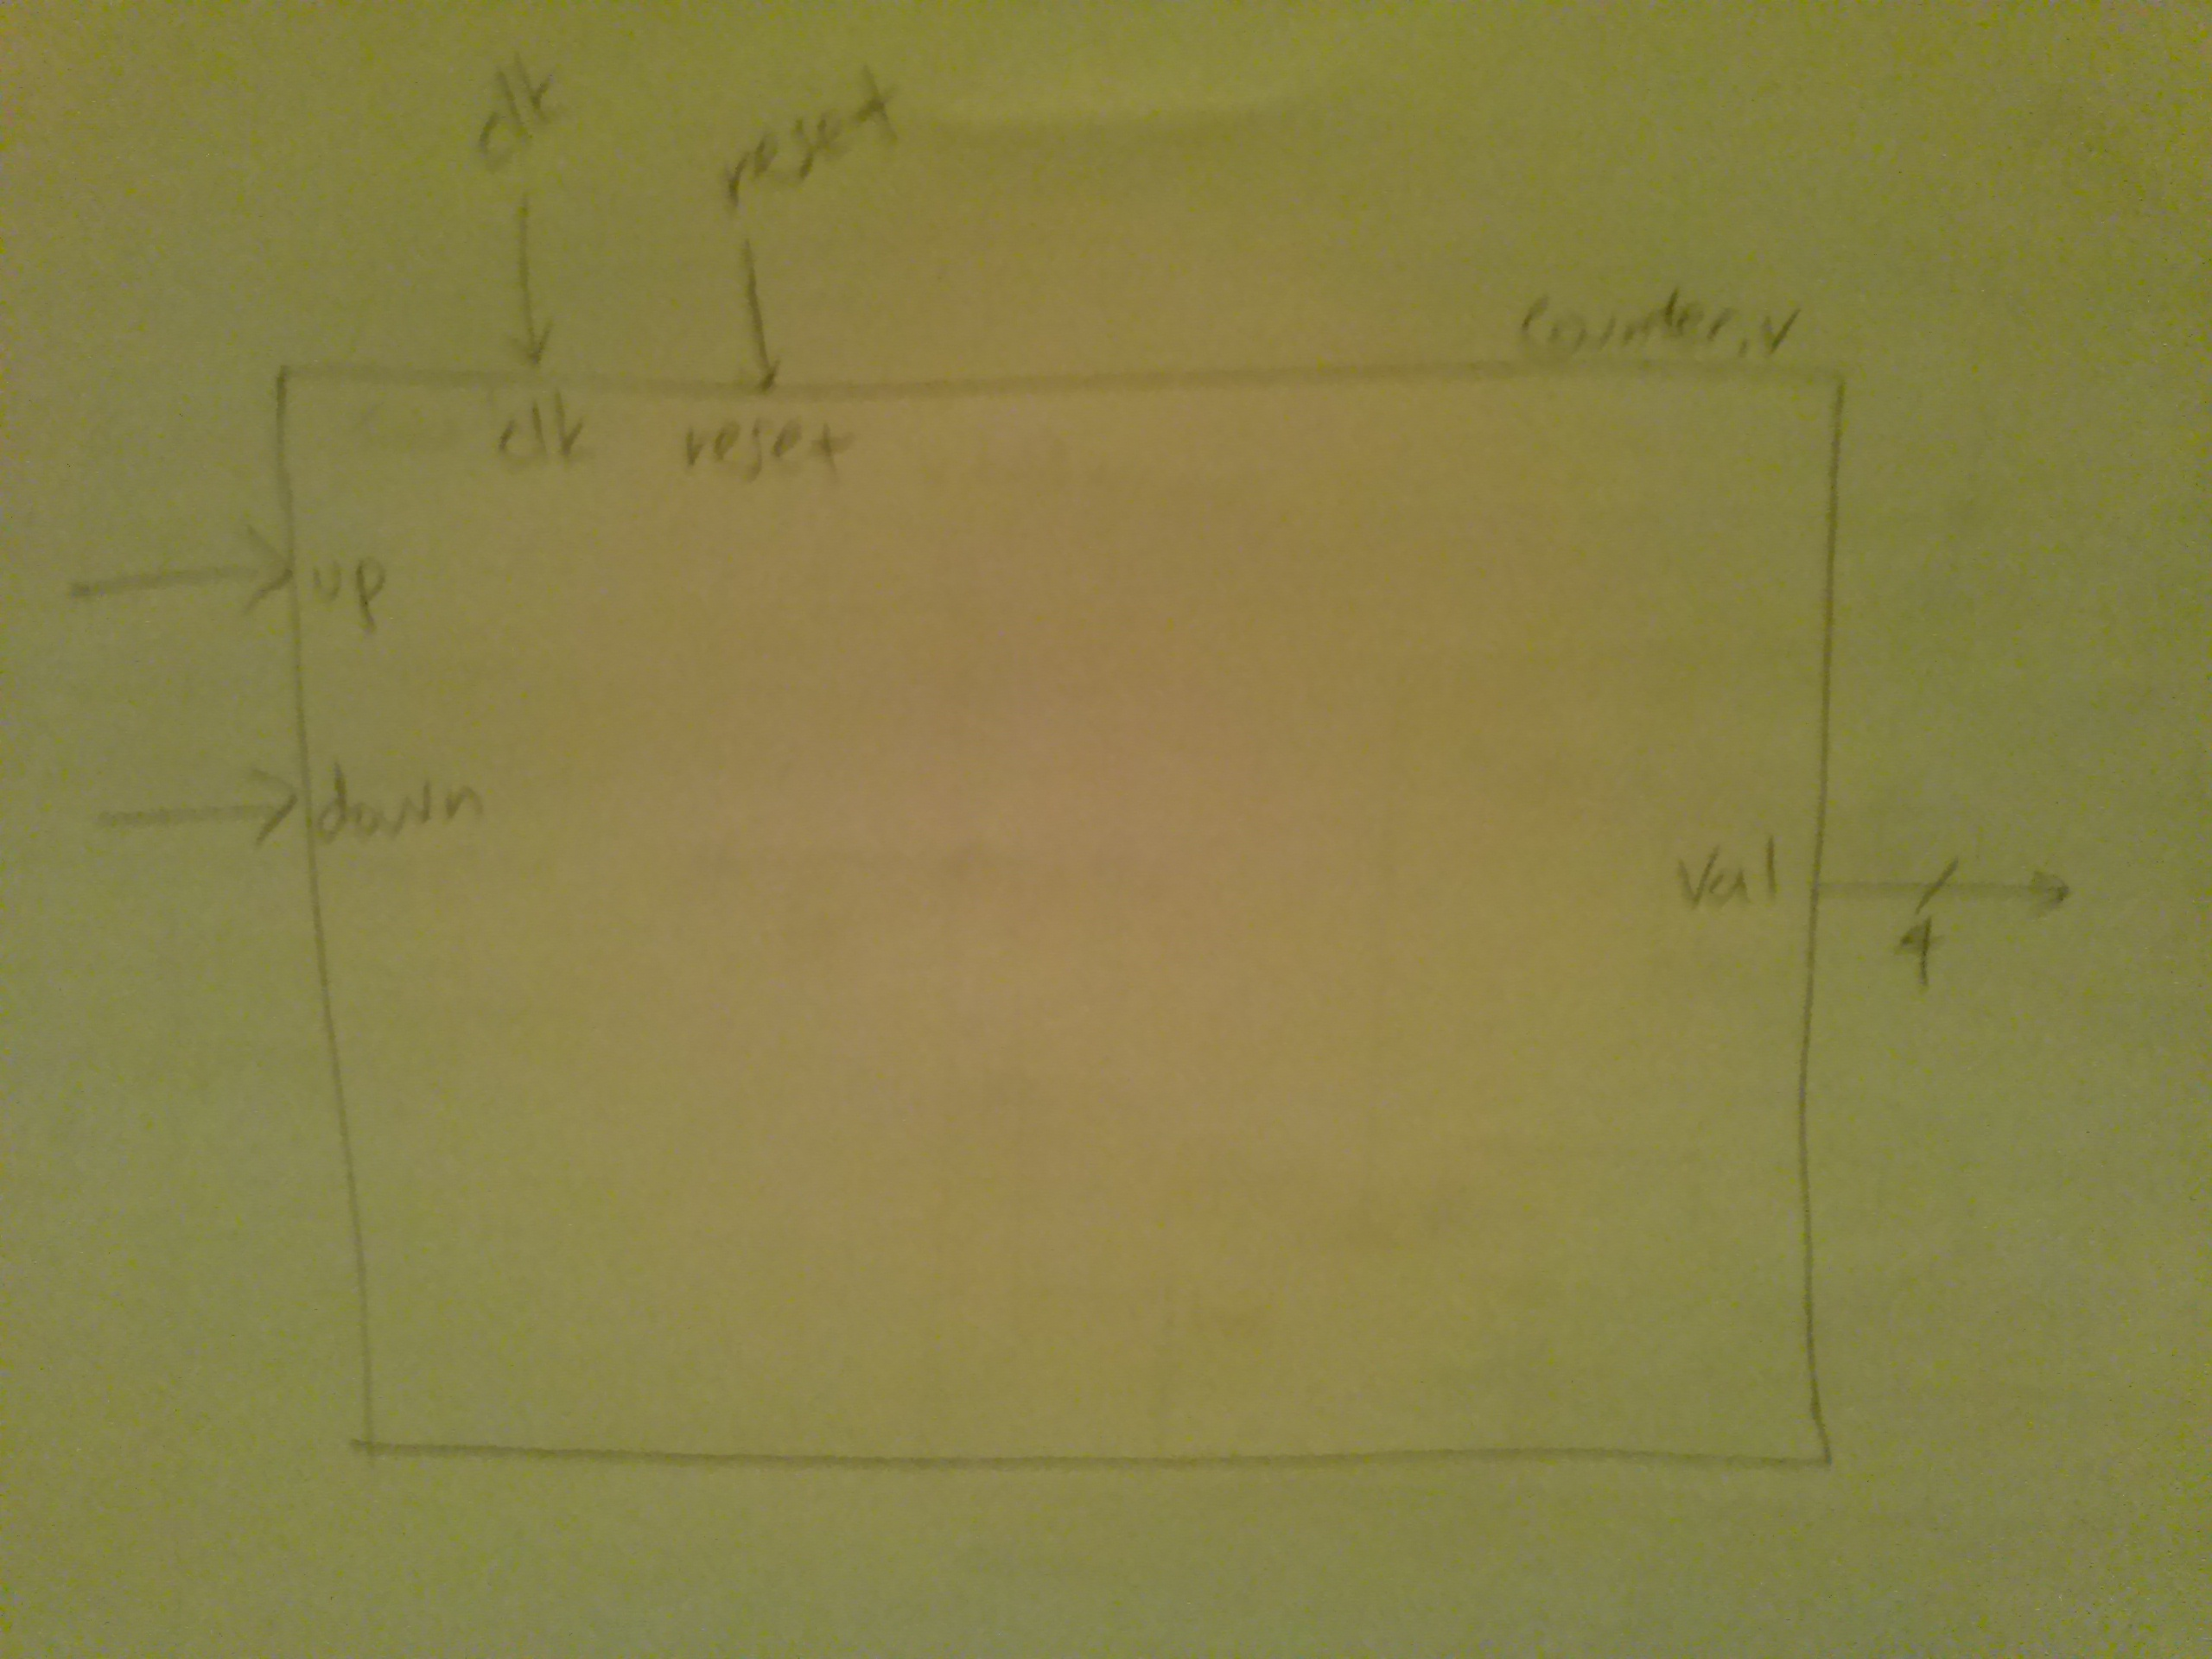
\includegraphics[width=0.75\linewidth]{figures/block_diagrams/counter.jpg}
        \caption{counter module block diagram}
        \label{fig:counter_blockdiagram}
      \end{figure}

      \begin{figure}[H]
        \centering
        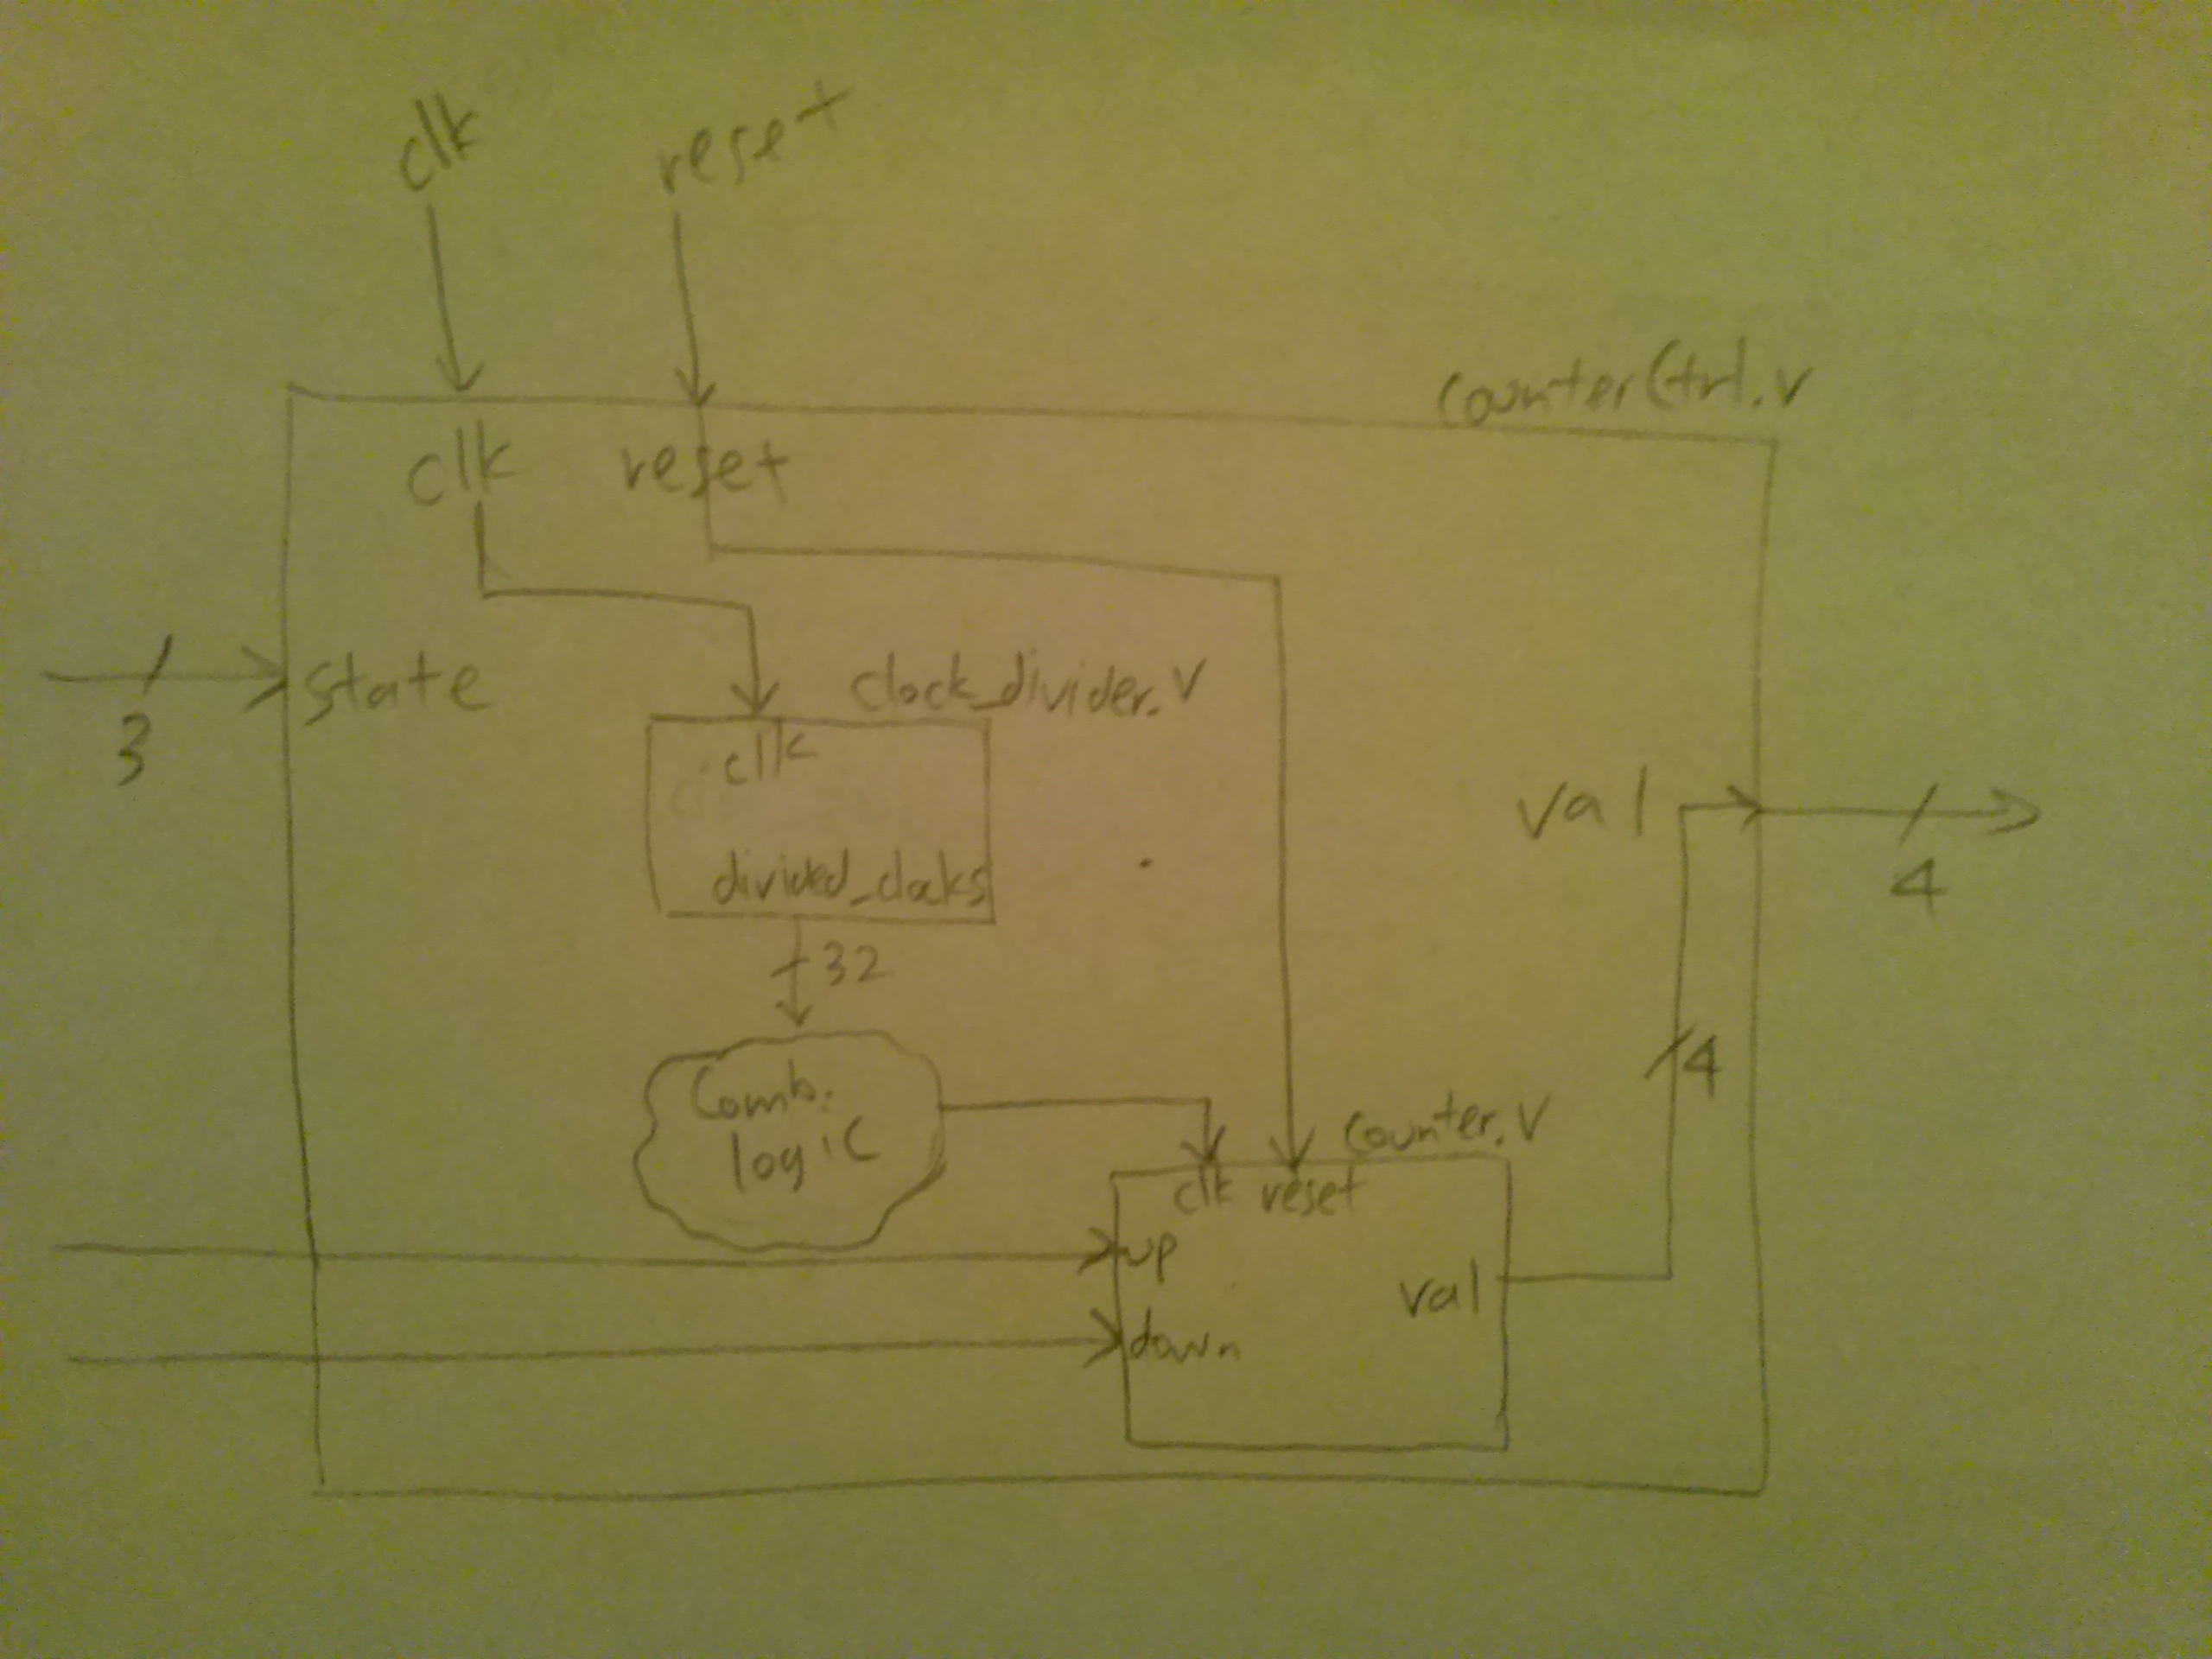
\includegraphics[width=0.75\linewidth]{figures/block_diagrams/counterCtrl.jpg}
        \caption{counterCtrl module block diagram}
        \label{fig:counterCtrl_blockdiagram}
      \end{figure}

      \begin{figure}[H]
        \centering
        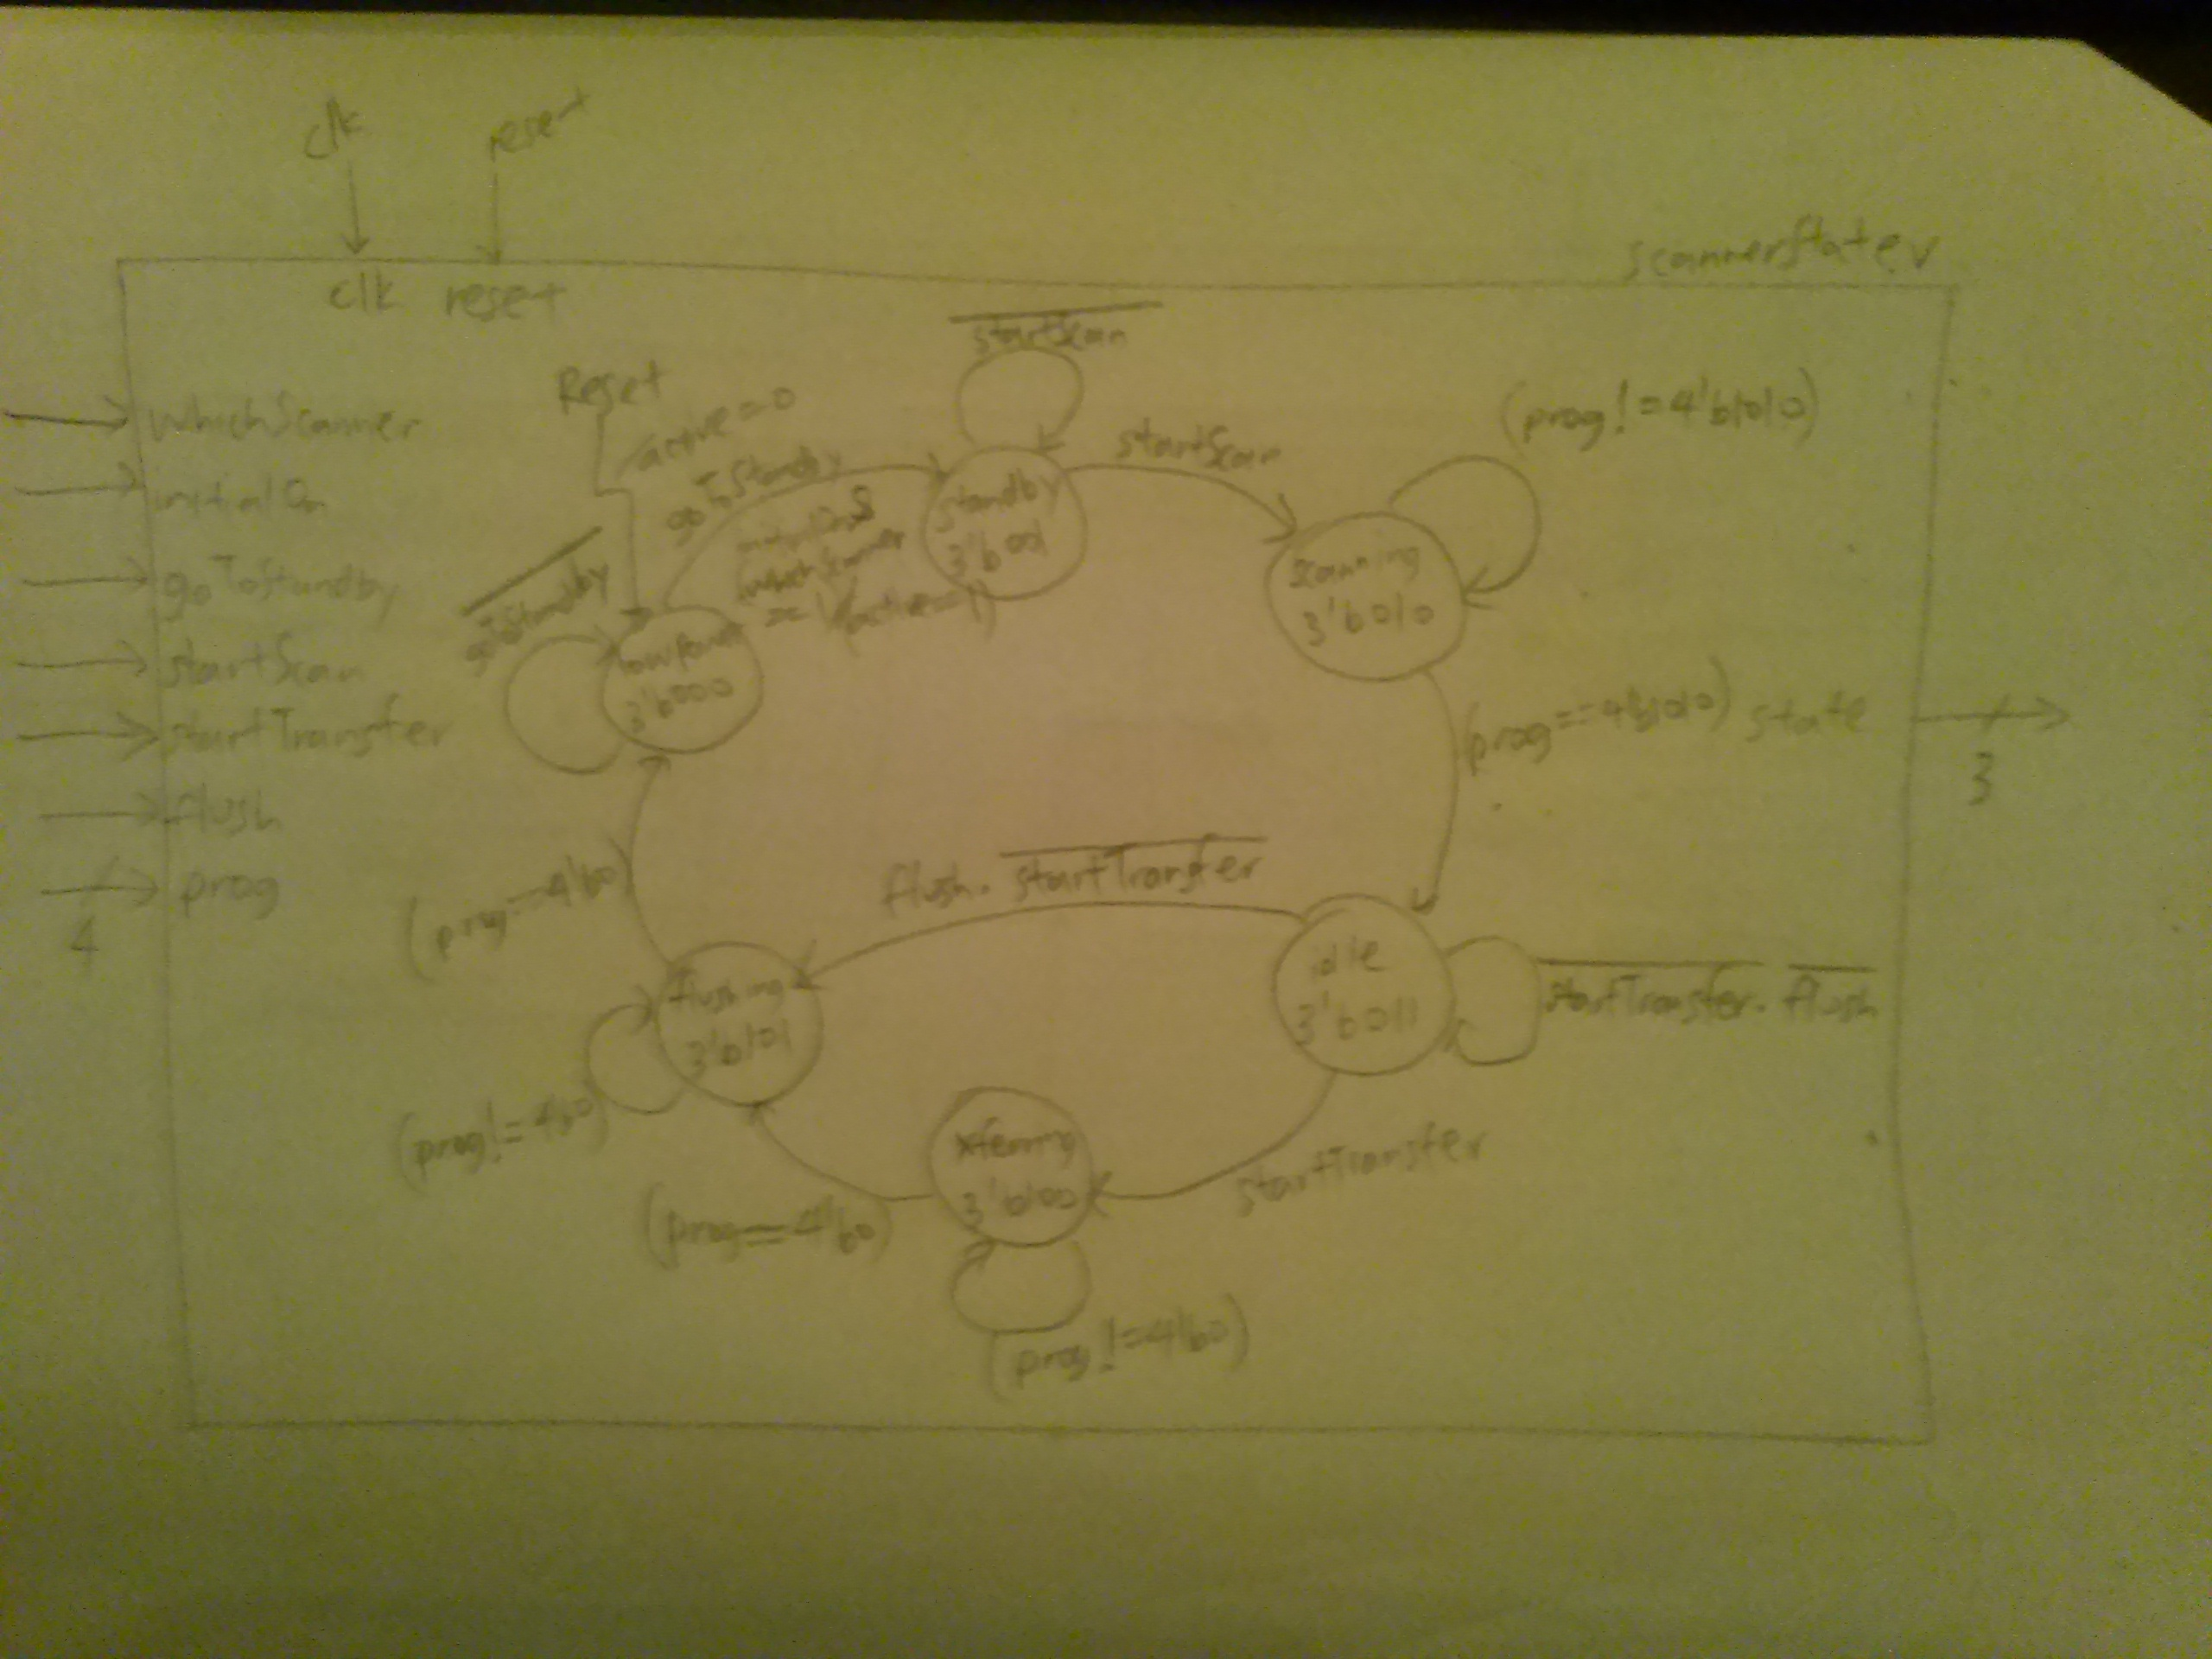
\includegraphics[width=0.75\linewidth]{figures/block_diagrams/scannerState.jpg}
        \caption{state transition diagram for the scanners}
        \label{fig:scannerState_FSM}
      \end{figure}

      \begin{figure}[H]
        \centering
        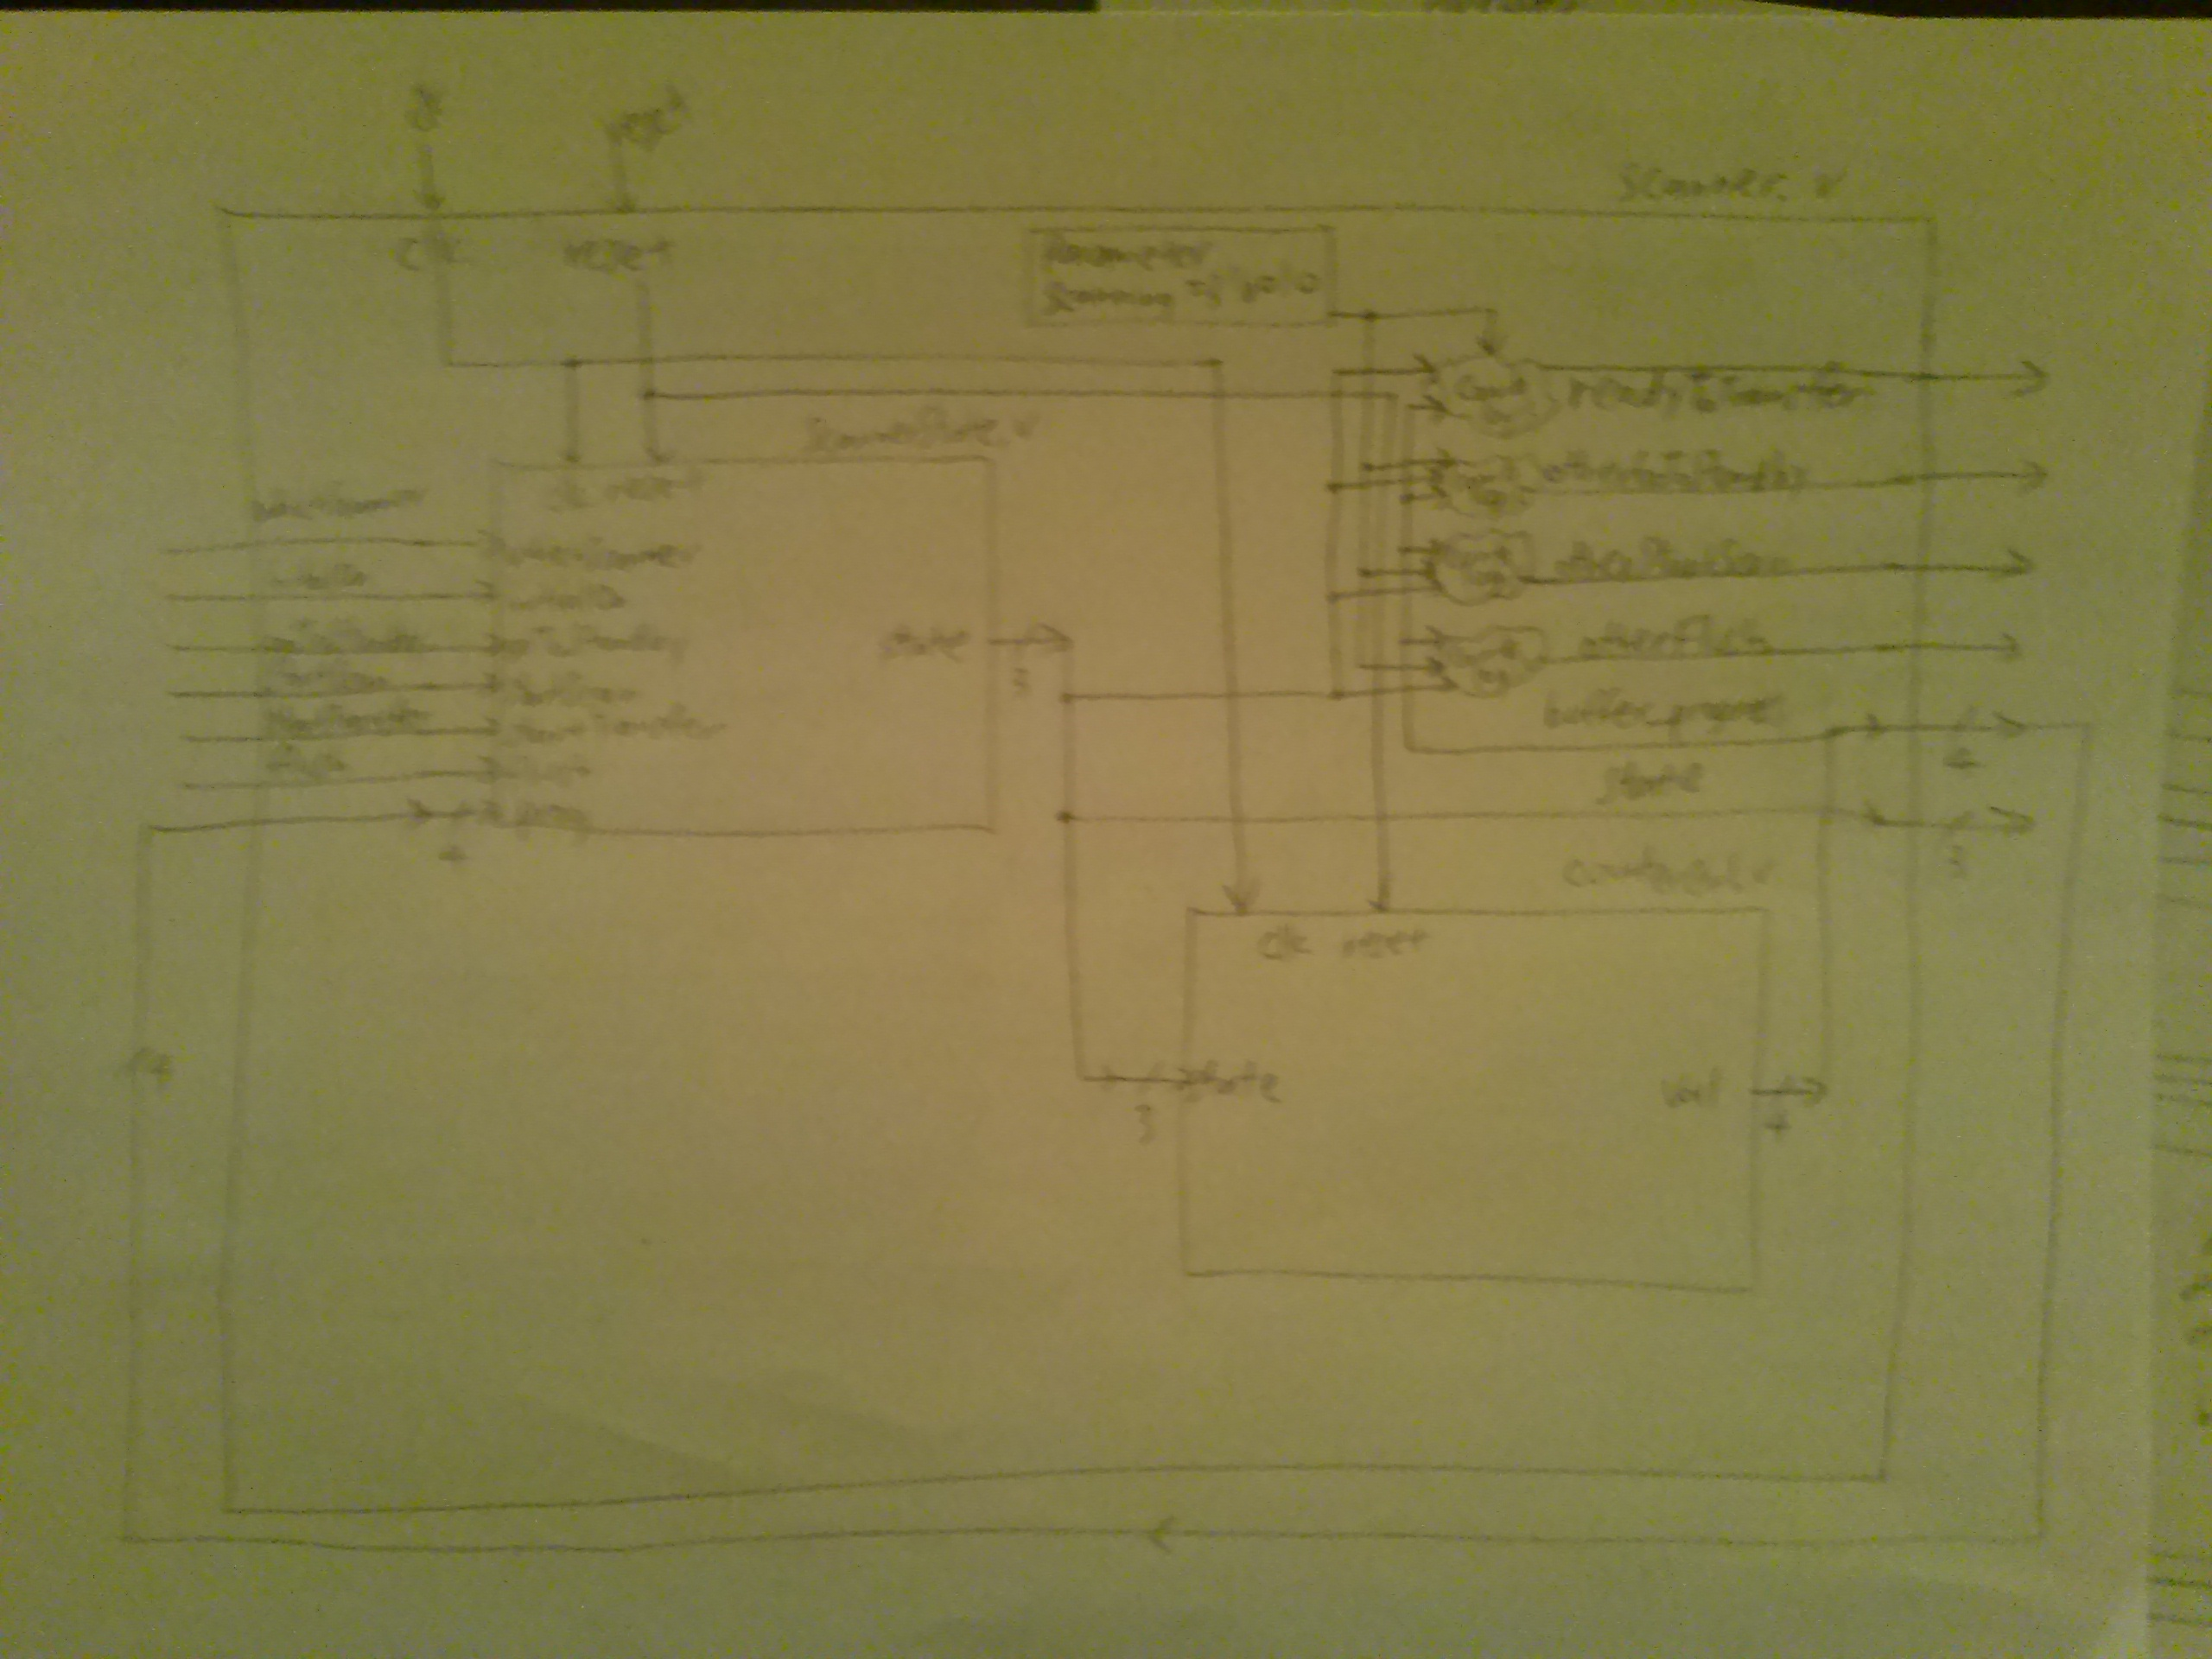
\includegraphics[width=0.75\linewidth]{figures/block_diagrams/scanner.jpg}
        \caption{scanner module block diagram}
        \label{fig:scanner_blockdiagram}
      \end{figure}

      \begin{figure}[H]
        \centering
        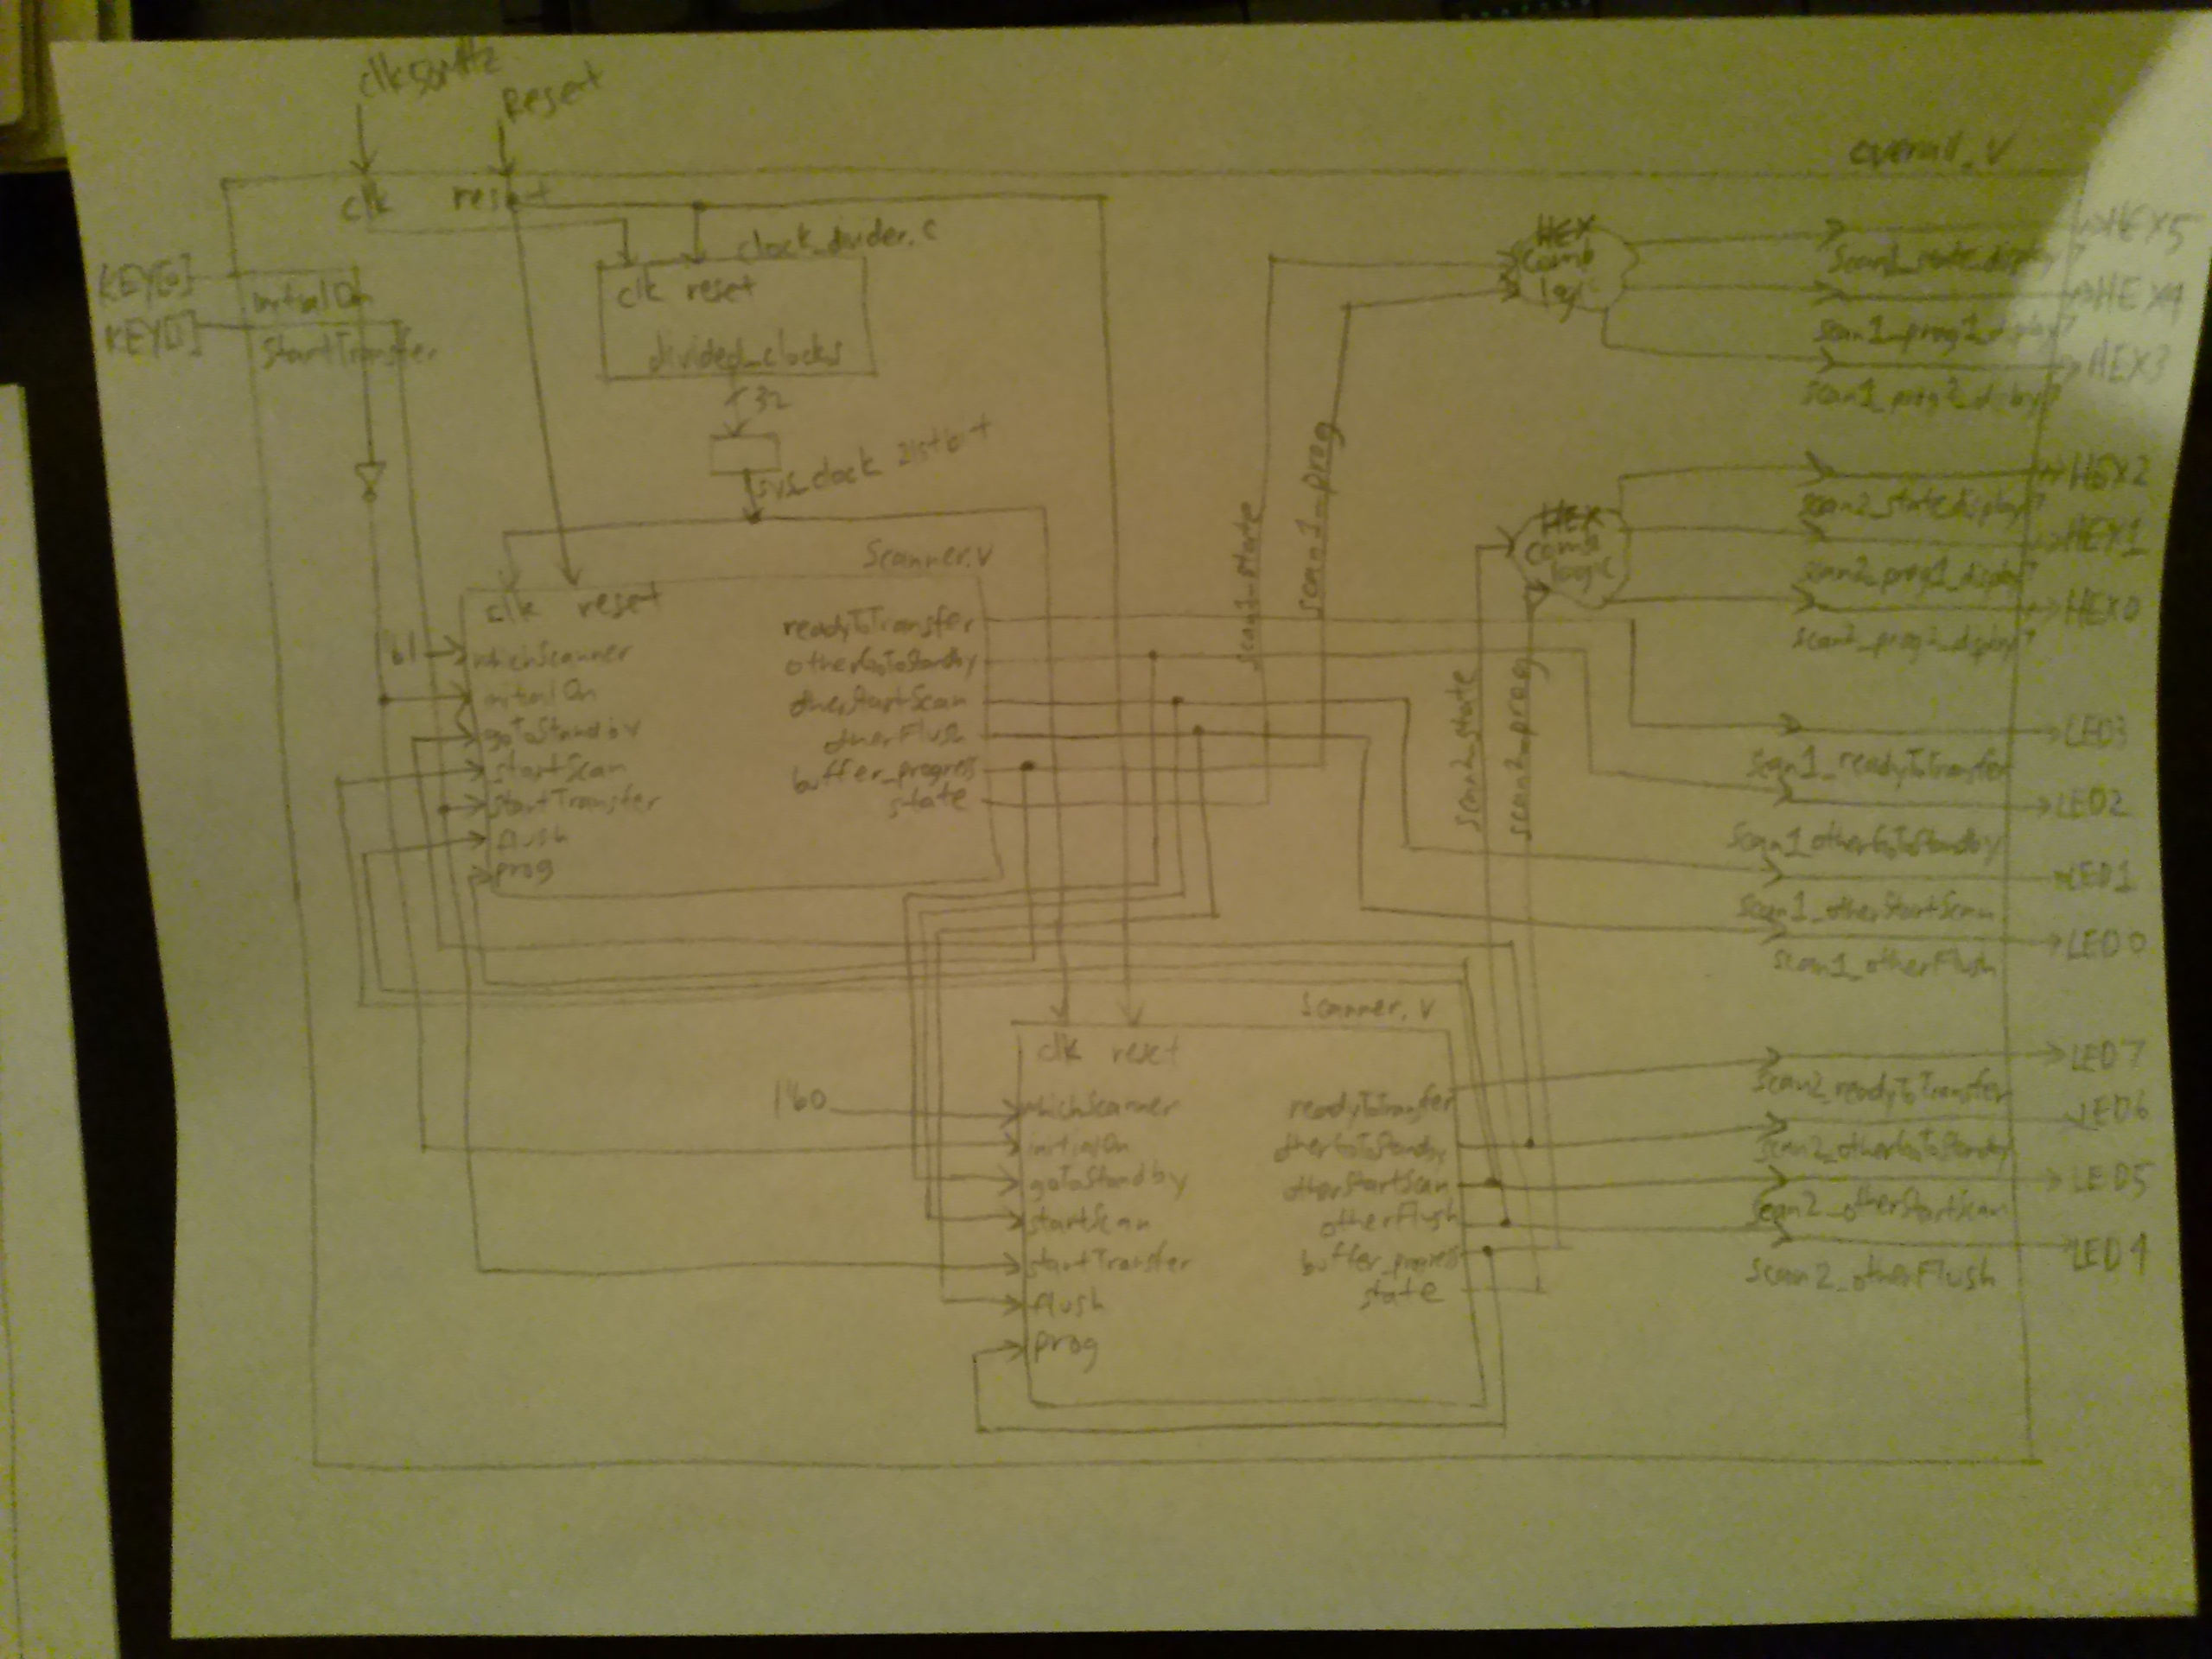
\includegraphics[width=0.75\linewidth]{figures/block_diagrams/lab4_overall_blockdiagram.jpg}
        \caption{overall module block diagram}
        \label{fig:lab4_overall_blockdiagram}
      \end{figure}

      \begin{figure}[H]
        \centering
        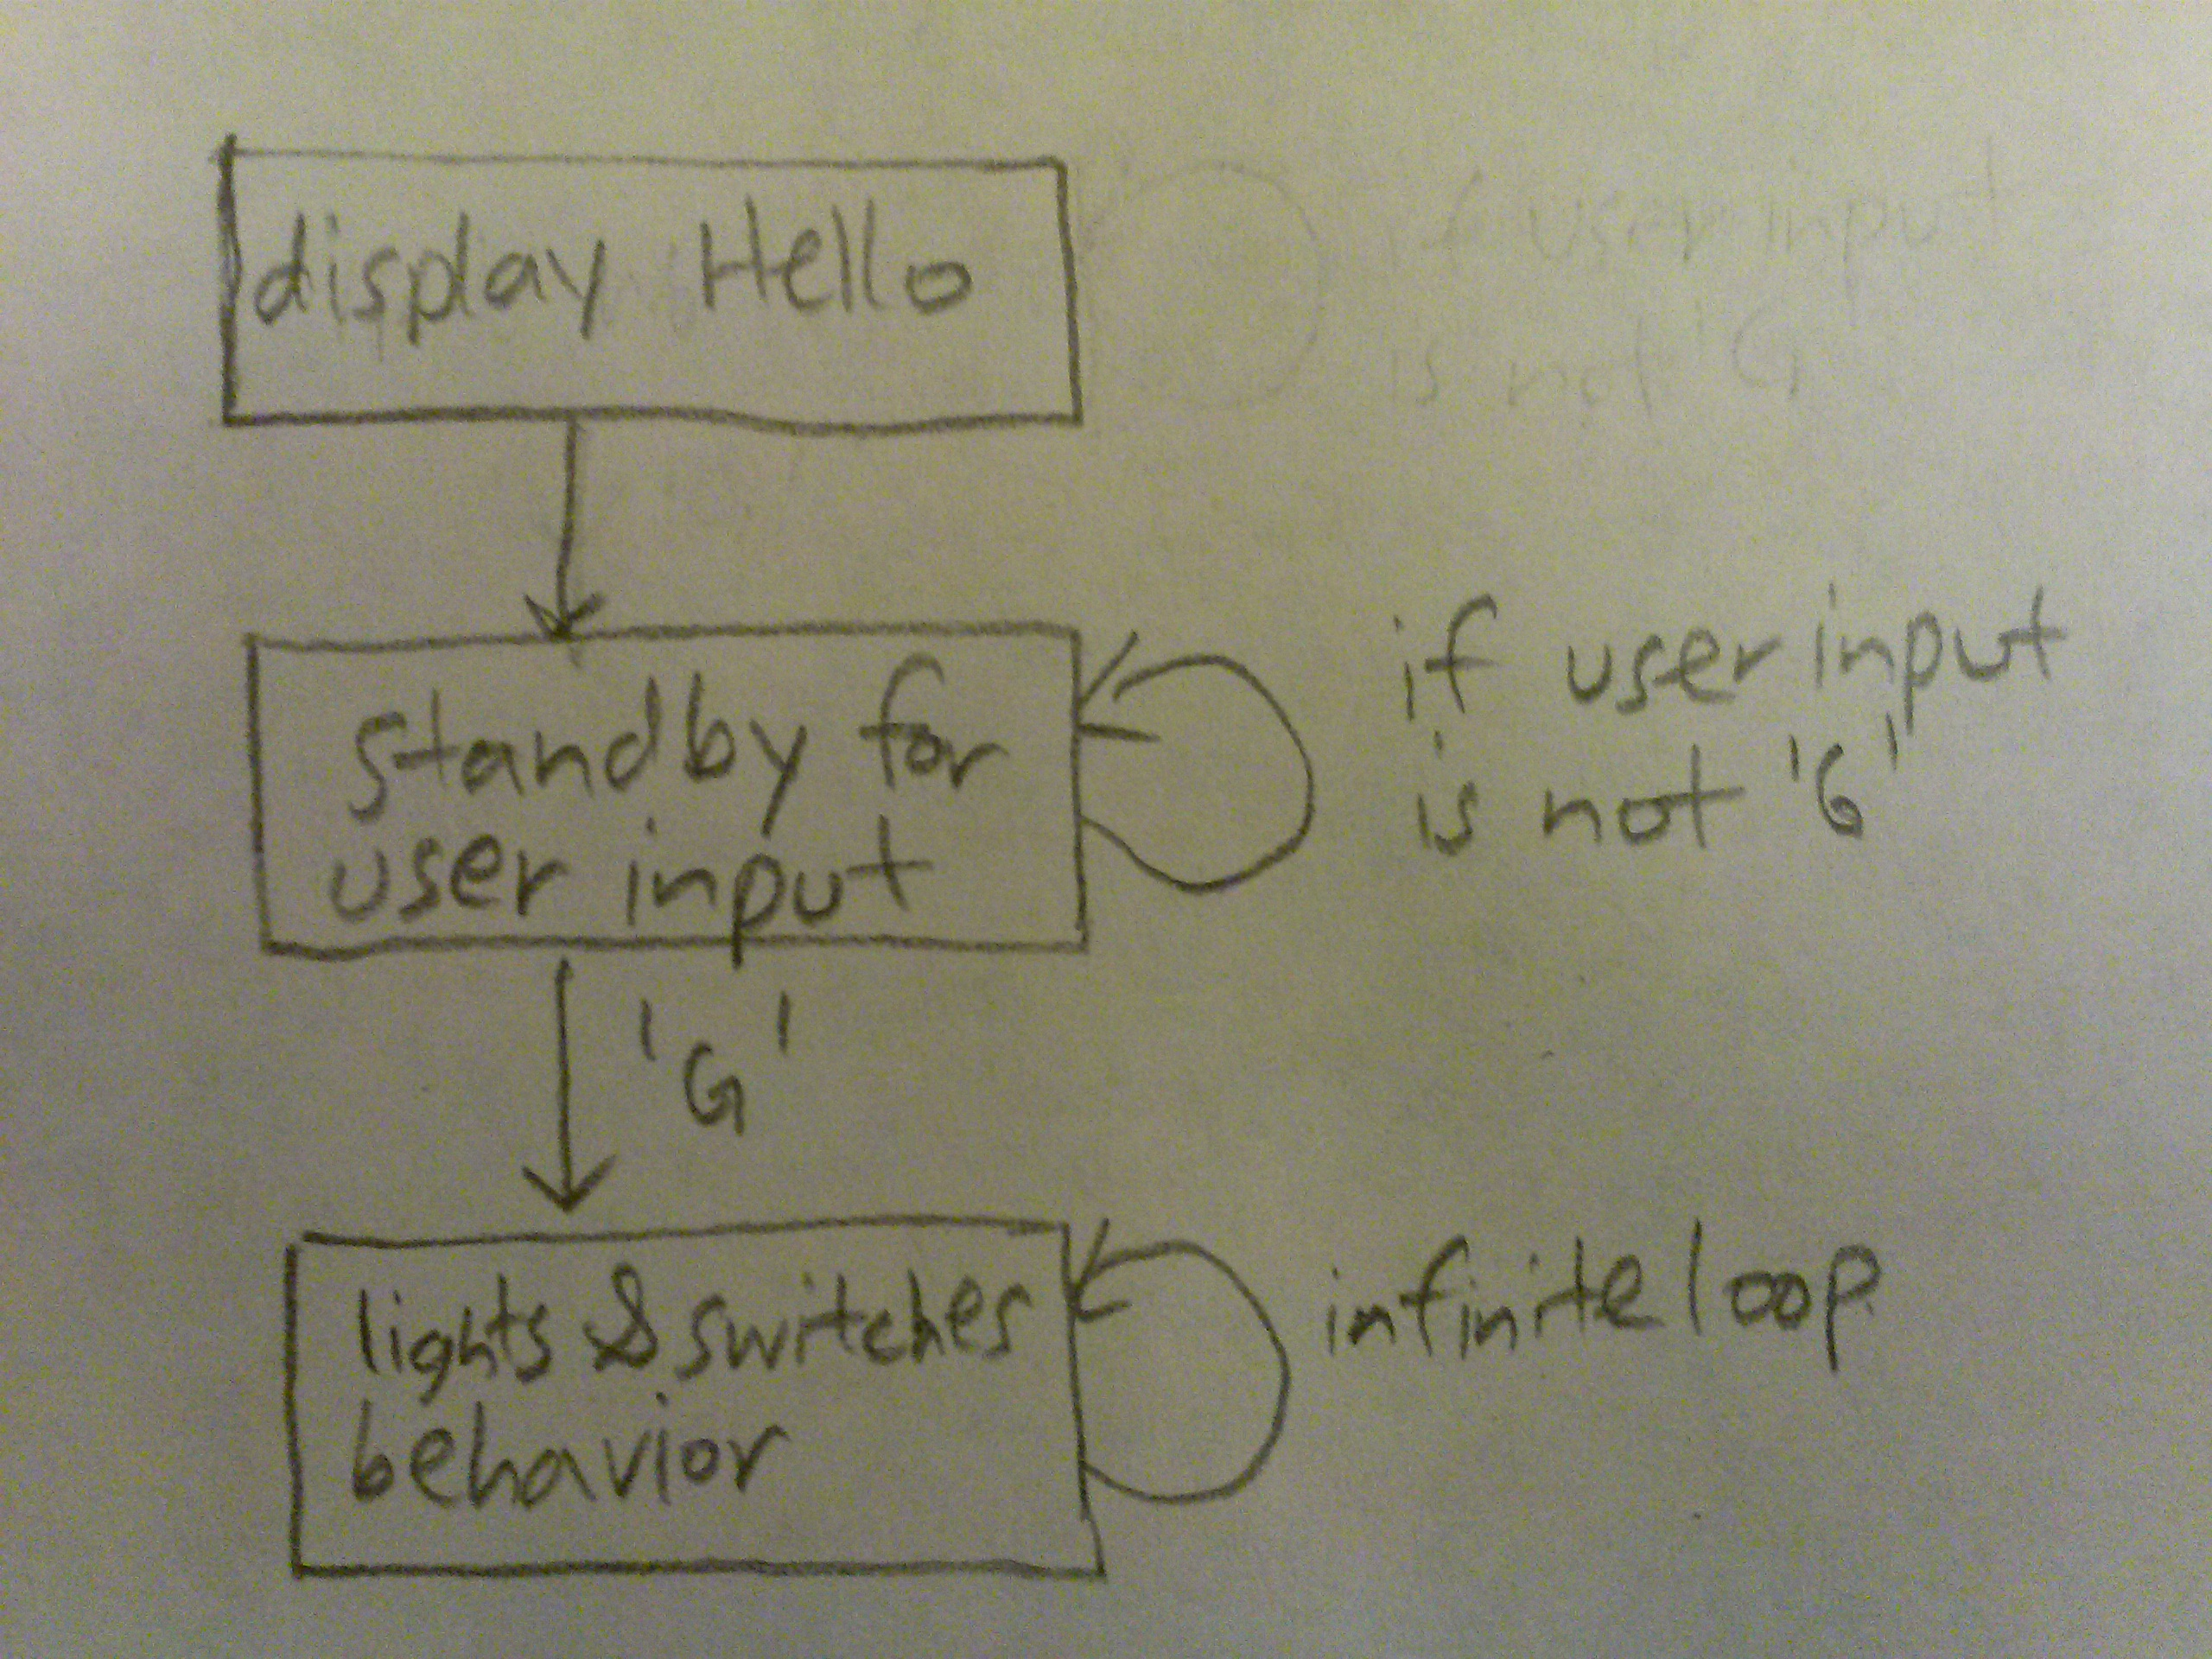
\includegraphics[width=0.75\linewidth]{figures/block_diagrams/lab4_lightsandswitchesmod_blockdiagram.jpg}
        \caption{modified lights and switches block diagram}
        \label{fig:ligthsandswitchesmod_blockdiagram}
      \end{figure}

      \begin{figure}[H]
        \centering
        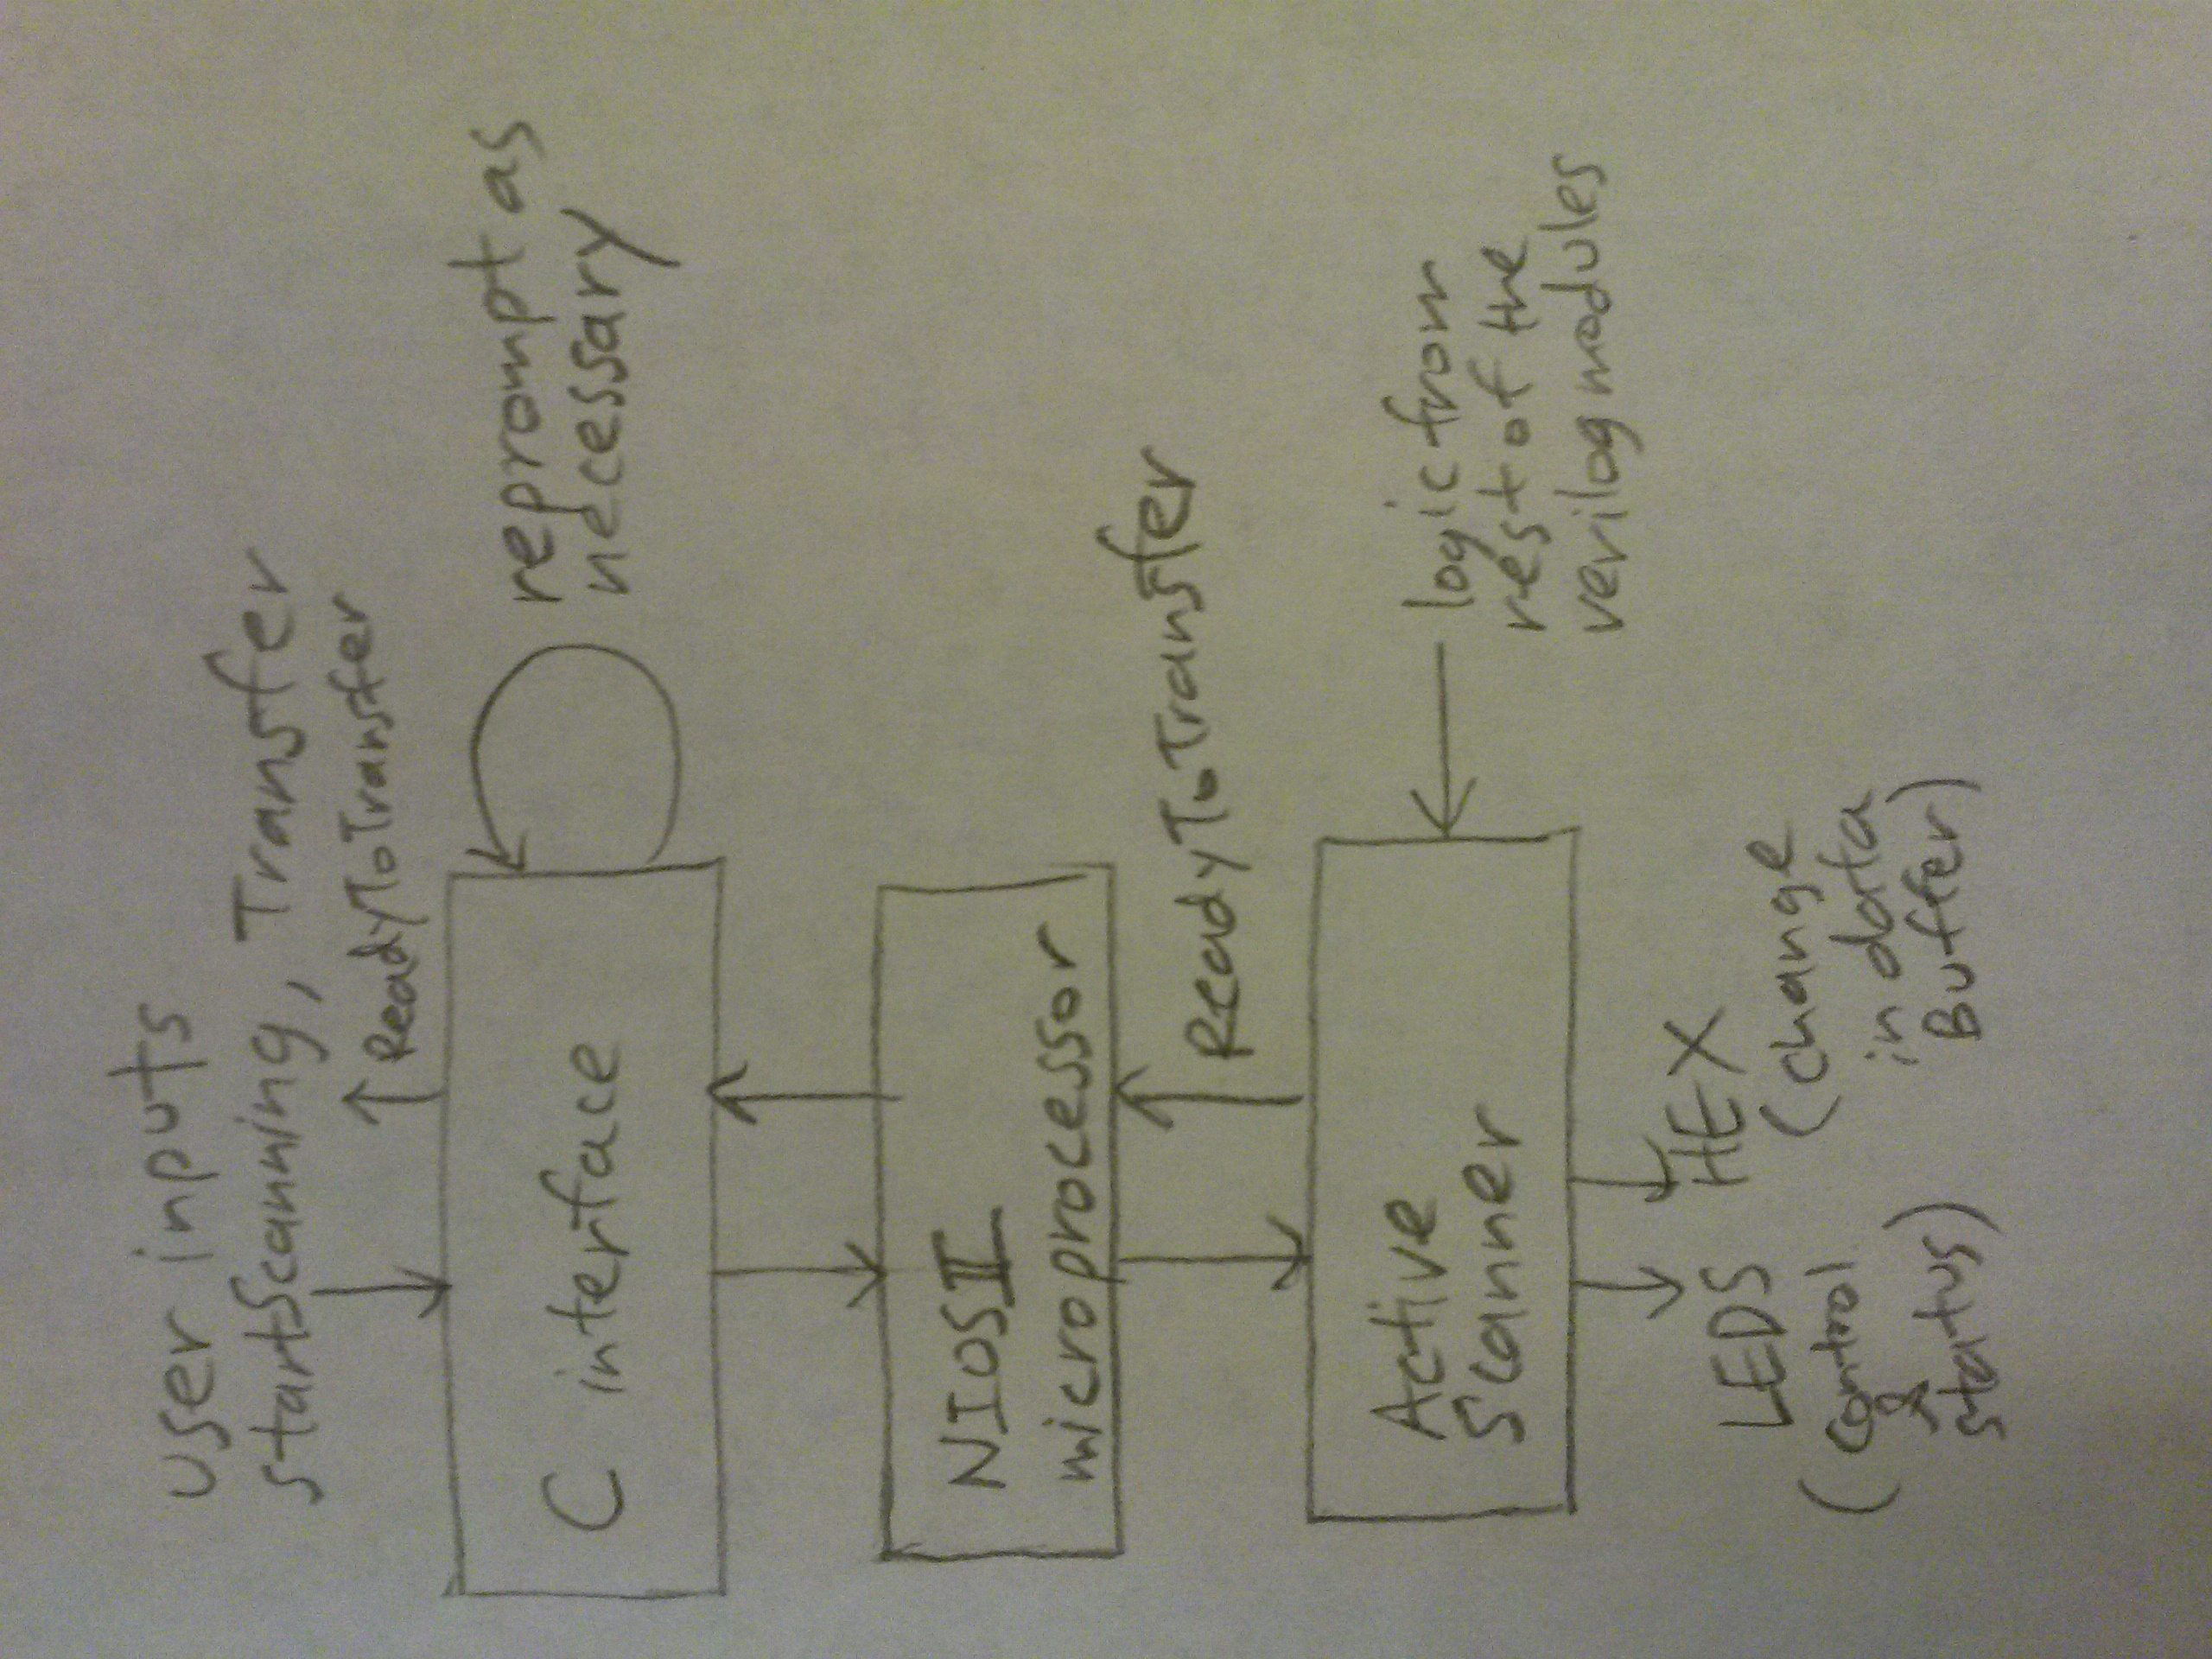
\includegraphics[width=0.75\linewidth]{figures/block_diagrams/lab4_scannerIO_blockdiagram.jpg}
        \caption{scannerIO user interface block diagram}
        \label{fig:scannerIO_blockdiagram}
      \end{figure}

    \subsubsection{Verilog}
      % counter.v
      \lstinputlisting[language=Verilog]{../verilog/scanner/counter.v}
      \lstinputlisting[language=Verilog]{../verilog/scanner/counter_testbench.v}

      % scannerState.v
      \lstinputlisting[language=Verilog]{../verilog/scanner/scannerState.v}
      \lstinputlisting[language=Verilog]{../verilog/scanner/scannerState_testbench.v}

      % dataBuffer.v
      \lstinputlisting[language=Verilog]{../verilog/scanner/dataBuffer.v}
      \lstinputlisting[language=Verilog]{../verilog/scanner/dataBuffer_testbench.v}

      % scanner.v
      \lstinputlisting[language=Verilog]{../verilog/scanner/scanner.v}
      \lstinputlisting[language=Verilog]{../verilog/scanner/scanner_testbench.v}

      % scannerIO.v
      \lstinputlisting[language=Verilog]{../verilog/scanner/lab4_scannerIO.v}

    \subsubsection{C Program}
      % countBinary.c
      \lstinputlisting[language=C]{../software/count_binary.c}

      % lights_and_switches
      \lstinputlisting[language=C]{../software/lights_and_switches.c}

      % lights_and_switches (mod)
      \lstinputlisting[language=C]{../software/lights_and_switches_mod.c}

      % scannerIO
      \lstinputlisting[language=C]{../software/scannerIO.c}

    \subsubsection{iverilog \& gtkwave}
      % counter gtkwave
      \begin{figure}[H]
        \centering
        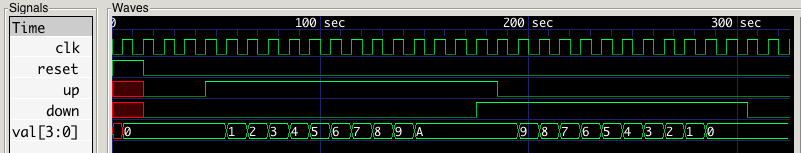
\includegraphics[width=0.75\linewidth]{figures/gtkwave/counter_gtkwave.png}
        \caption{counter module waveform}
        \label{fig:counter_gtkwave}
      \end{figure}

      % counterCtrl gtkwave
      \begin{figure}[H]
        \centering
        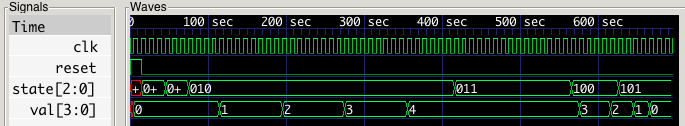
\includegraphics[width=0.75\linewidth]{figures/gtkwave/counterCtrl_gtkwave.png}
        \caption{counterCtrl module waveform}
        \label{fig:counterCtrl_gtkwave}
      \end{figure}

      % scannerState gtkwave
      \begin{figure}[H]
        \centering
        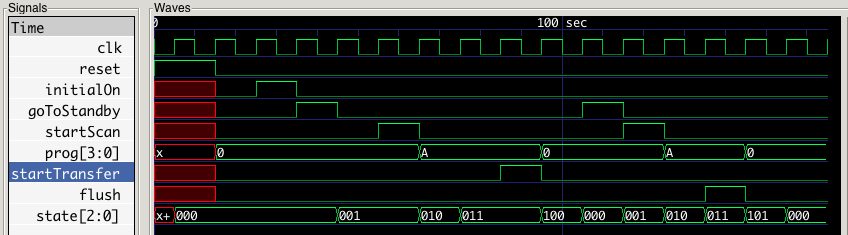
\includegraphics[width=0.75\linewidth]{figures/gtkwave/scannerState_gtkwave.png}
        \caption{scannerState module waveform}
        \label{fig:scannerState_gtkwave}
      \end{figure}

      % scanner gtkwave
      \begin{figure}[H]
        \centering
        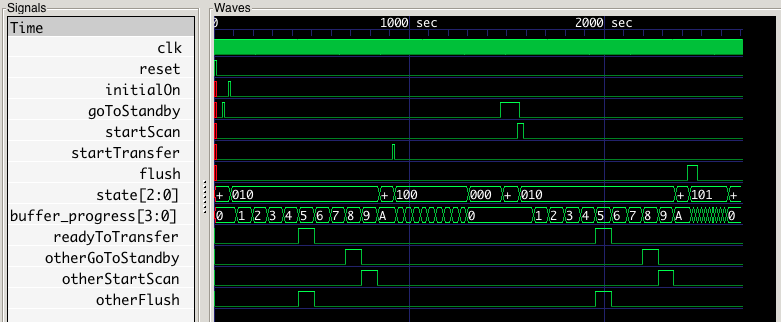
\includegraphics[width=0.75\linewidth]{figures/gtkwave/scanner_gtkwave.png}
        \caption{scanner module waveform}
        \label{fig:scanner_gtkwave}
      \end{figure}

      % overall gtkwave
      \begin{figure}[H]
        \centering
        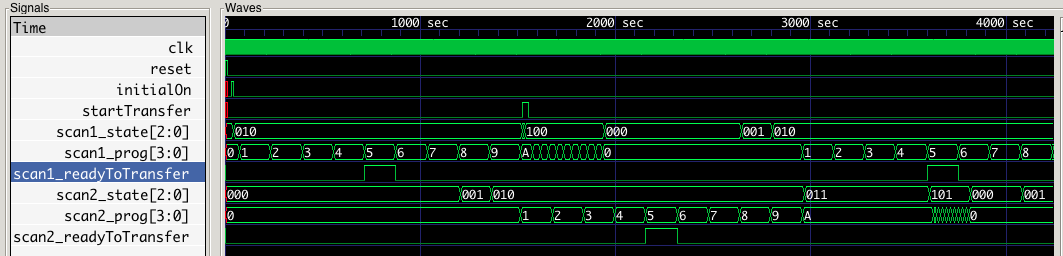
\includegraphics[width=0.75\linewidth]{figures/gtkwave/overall_gtkwave.png}
        \caption{overall module waveform}
        \label{fig:overall_gtkwave}
      \end{figure}

    \subsubsection{Miscellaneous}
      \begin{figure}[H]
        \centering
        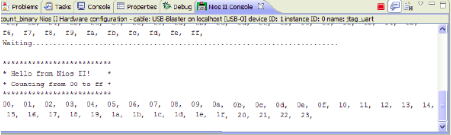
\includegraphics[width=0.75\linewidth]{figures/countbinary_output.png}
        \caption{countbinary output}
        \label{fig:countbinary_output}
      \end{figure}

      \begin{figure}[H]
        \centering
        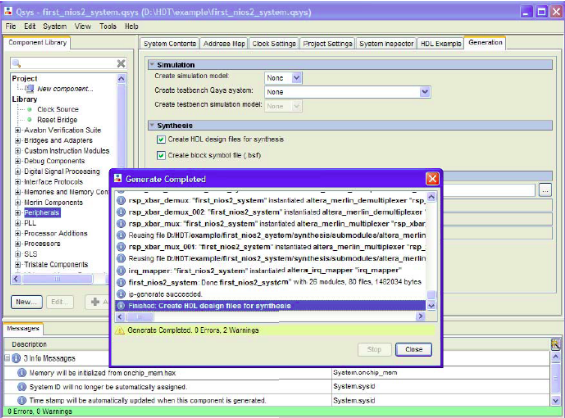
\includegraphics[width=0.75\linewidth]{figures/qsys_generate.png}
        \caption{using qsys to generate a NIOS II processor}
        \label{fig:qsys_generate}
      \end{figure}

  \subsection{Lab 5}
    \subsubsection{Block Diagrams}
      \begin{figure}[H]
        \centering
        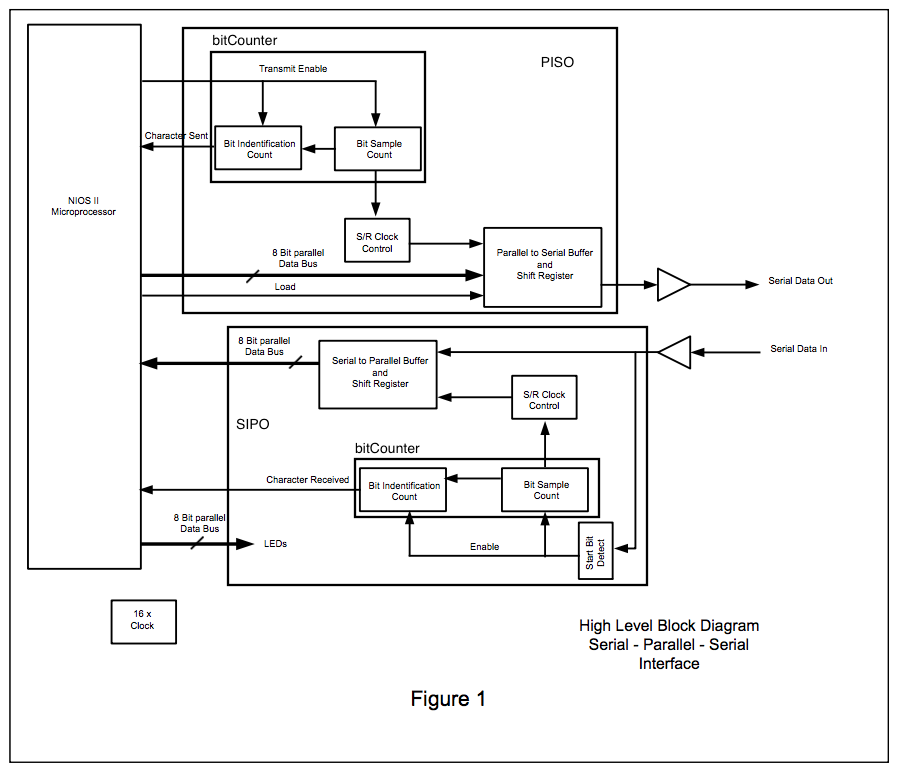
\includegraphics[width=0.75\linewidth]{figures/block_diagrams/SPS_interface_blockdiagram.png}
        \caption{SPS\_interface module block diagram}
        \label{fig:SPS_interface_blockdiagram}
      \end{figure}

      \begin{figure}[H]
        \centering
        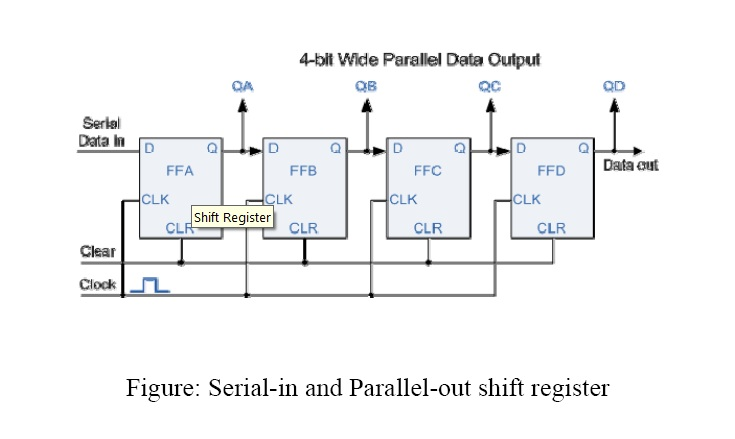
\includegraphics[width=0.75\linewidth]{figures/block_diagrams/spShiftReg_blockdiagram.jpg}
        \caption{spShiftReg module block diagram}
        \label{fig:spShiftReg_blockdiagram}
      \end{figure}

      \begin{figure}[H]
        \centering
        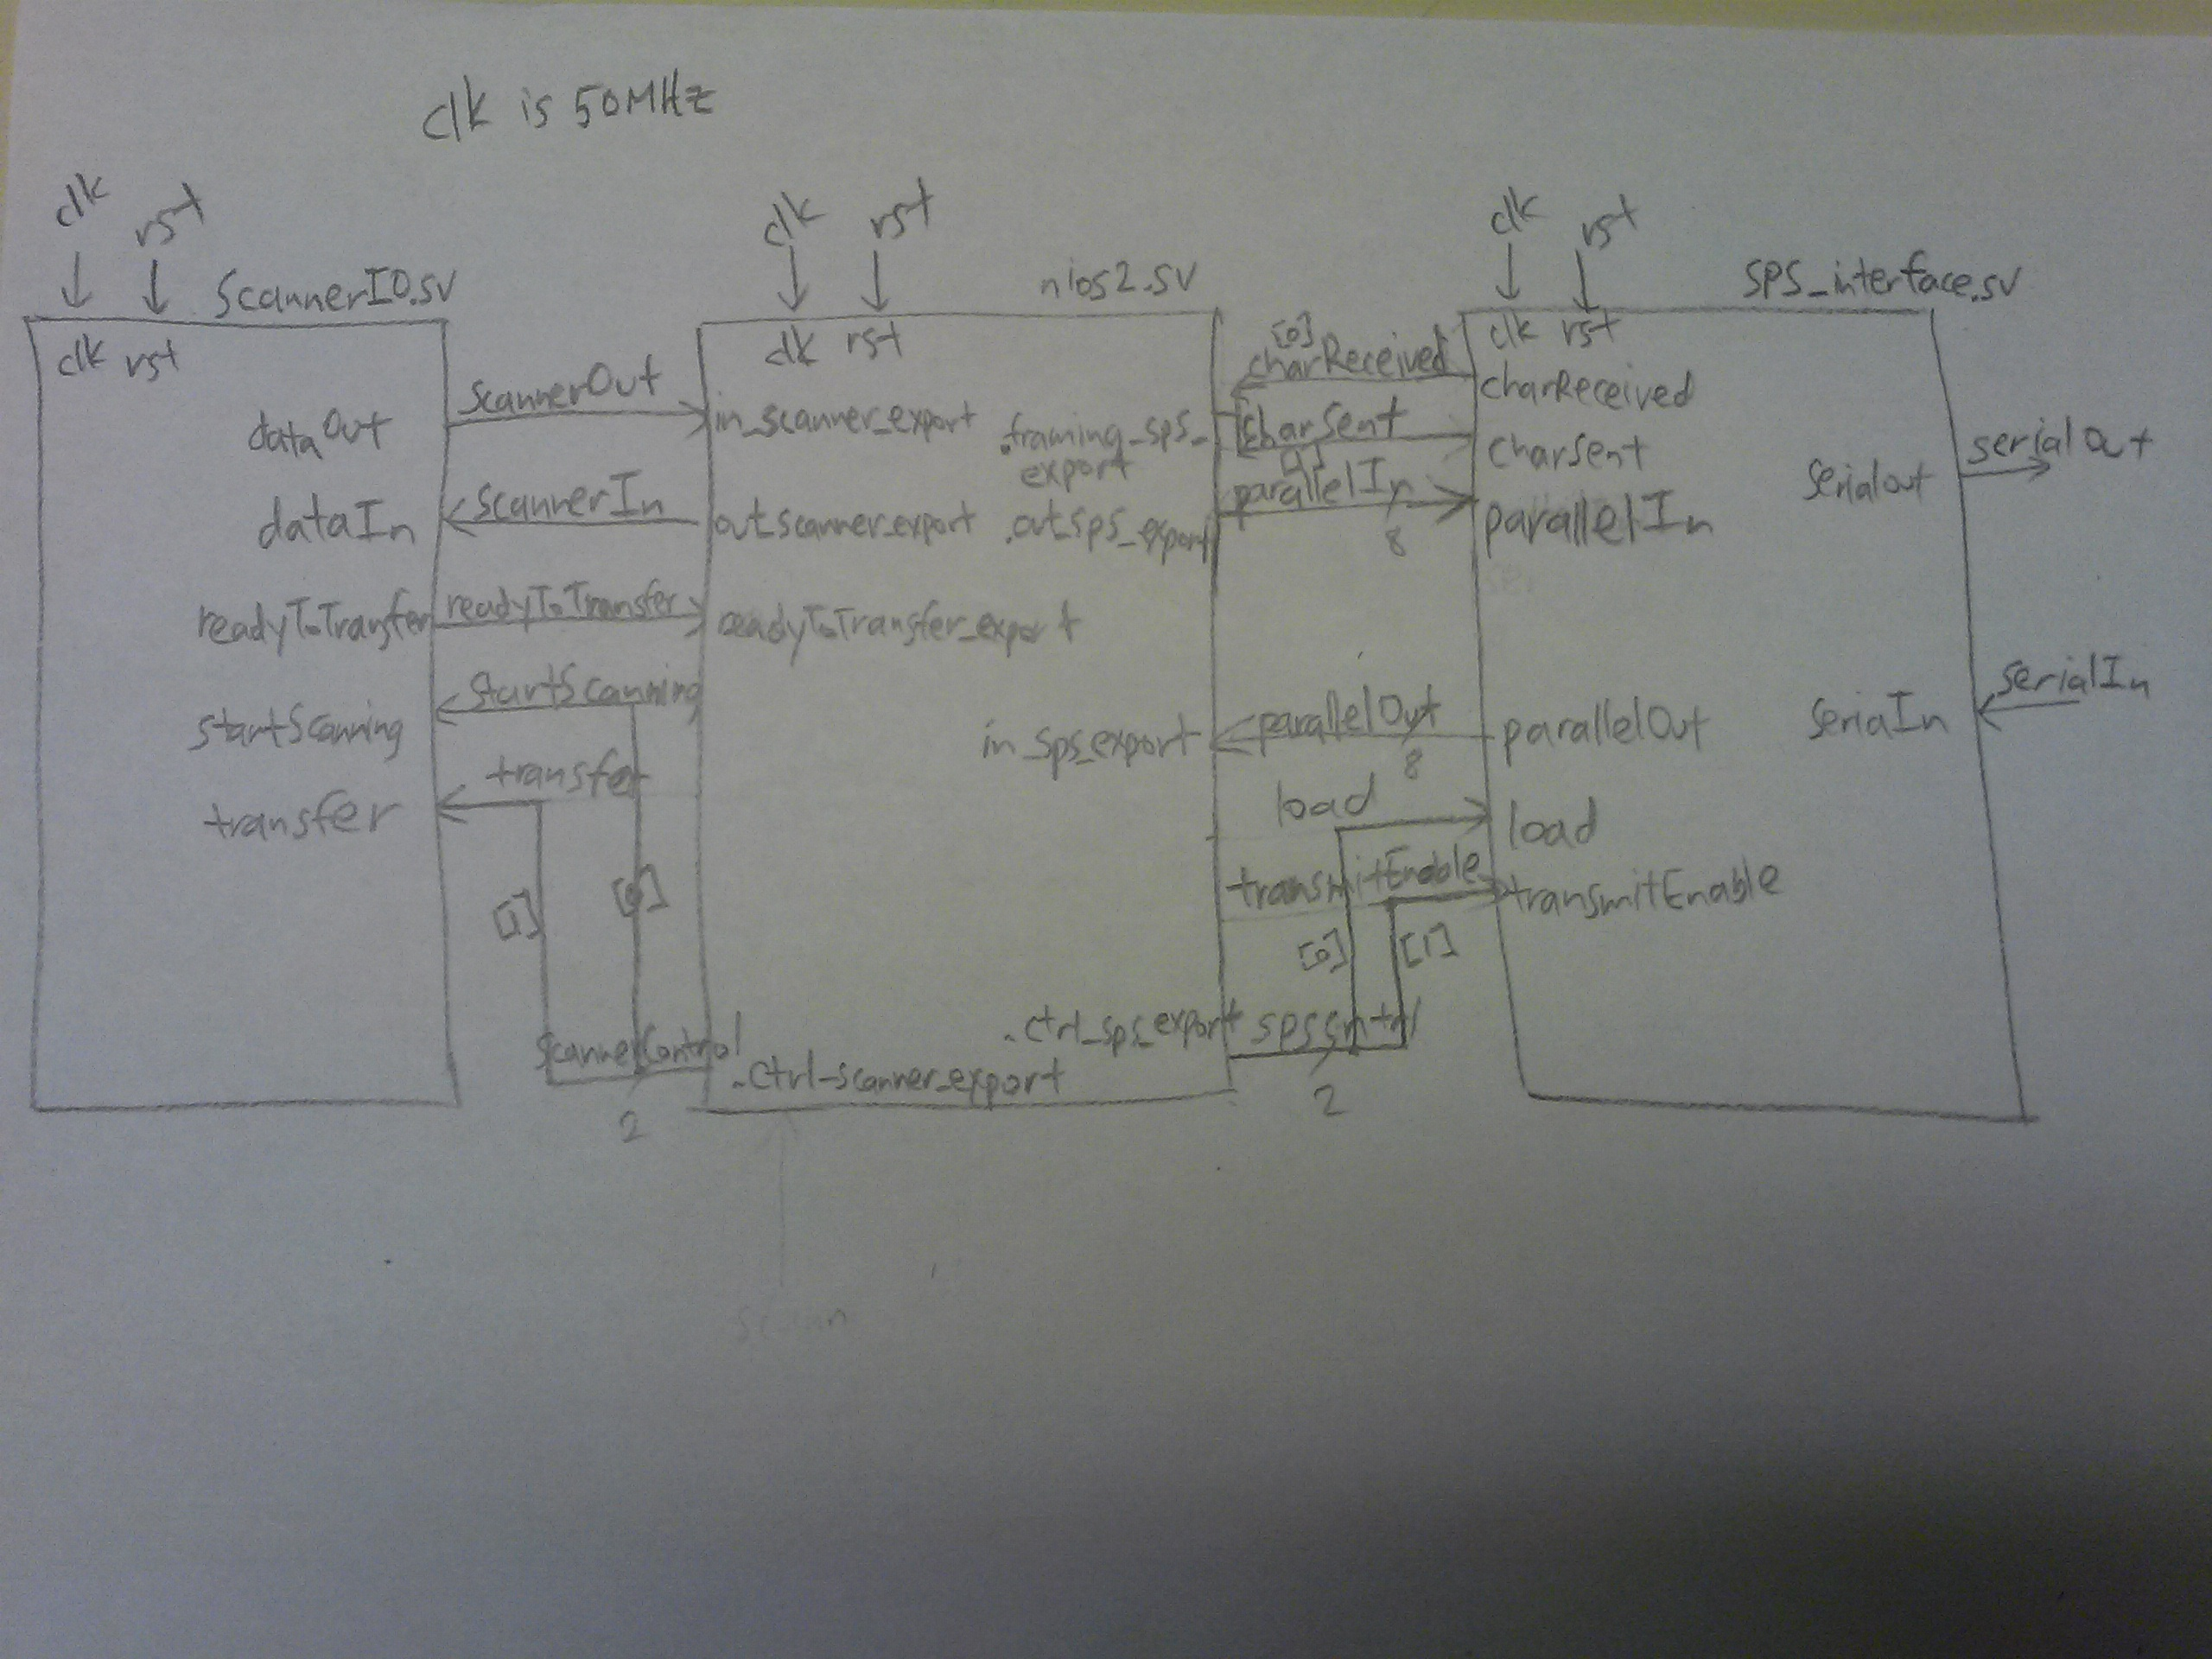
\includegraphics[width=0.75\linewidth]{figures/block_diagrams/overall_blockdiagram.jpg}
        \caption{overall scanner/home base module block diagram}
        \label{fig:lab5_overall_blockdiagram}
      \end{figure}

    \subsubsection{Verilog}
      % bsc.v
      \lstinputlisting[language=Verilog]{../verilog/SPS_interface/bsc.v}
      \lstinputlisting[language=Verilog]{../verilog/SPS_interface/bsc_testbench.v}

      % bic.v
      \lstinputlisting[language=Verilog]{../verilog/SPS_interface/bic.v}
      \lstinputlisting[language=Verilog]{../verilog/SPS_interface/bic_testbench.v}

      % bitCounter.v
      \lstinputlisting[language=Verilog]{../verilog/SPS_interface/bitCounter.v}
      \lstinputlisting[language=Verilog]{../verilog/SPS_interface/bitCounter_testbench.v}

      % psShiftReg.v
      \lstinputlisting[language=Verilog]{../verilog/SPS_interface/psShiftReg.v}
      \lstinputlisting[language=Verilog]{../verilog/SPS_interface/psShiftReg_testbench.v}

      % spShiftReg.v
      \lstinputlisting[language=Verilog]{../verilog/SPS_interface/spShiftReg.v}
      \lstinputlisting[language=Verilog]{../verilog/SPS_interface/spShiftReg_testbench.v}

      % PISO.v
      \lstinputlisting[language=Verilog]{../verilog/SPS_interface/PISO.v}
      \lstinputlisting[language=Verilog]{../verilog/SPS_interface/PISO_testbench.v}

      % SIPO.v
      \lstinputlisting[language=Verilog]{../verilog/SPS_interface/SIPO.v}
      \lstinputlisting[language=Verilog]{../verilog/SPS_interface/SIPO_testbench.v}

      % SPS_interface.v
      \lstinputlisting[language=Verilog]{../verilog/SPS_interface/SPS_interface.v}
      \lstinputlisting[language=Verilog]{../verilog/SPS_interface/SPS_interface_testbench.v}

      % overall.v
      \lstinputlisting[language=Verilog]{../verilog/overall.v}

      % overall.v
      \lstinputlisting[language=Verilog]{../verilog/displayToHex.v}
      \lstinputlisting[language=Verilog]{../verilog/displayToHex_testbench.v}

    \subsubsection{C Program}
      % scannerIO
      \lstinputlisting[language=C]{../software/hello_world_small.c}

      % smoke test
      \lstinputlisting[language=C]{../software/smoke_test.c}

    \subsubsection{iverilog \& gtkwave}
      % bsc
      \begin{figure}[H]
        \centering
        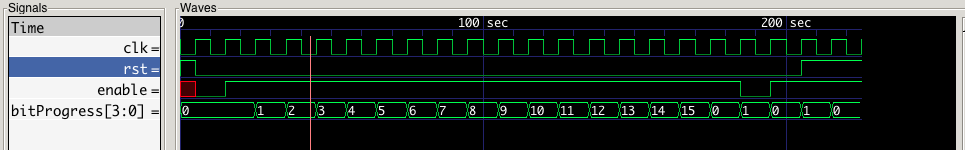
\includegraphics[width=0.75\linewidth]{figures/gtkwave/bsc_gtkwave.png}
        \caption{bsc module waveform}
        \label{fig:bsc_gtkwave}
      \end{figure}

      % bic
      \begin{figure}[H]
        \centering
        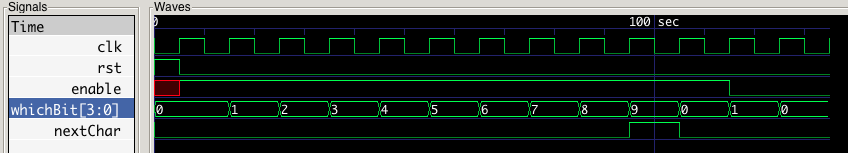
\includegraphics[width=0.75\linewidth]{figures/gtkwave/bic_gtkwave.png}
        \caption{bic module waveform}
        \label{fig:bic_gtkwave}
      \end{figure}

      % bitCounter
      \begin{figure}[H]
        \centering
        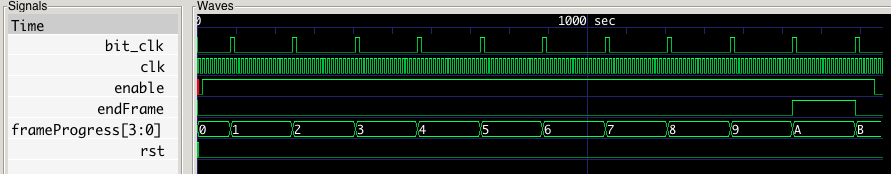
\includegraphics[width=0.75\linewidth]{figures/gtkwave/bitCounter_gtkwave.png}
        \caption{bitCounter module waveform}
        \label{fig:bitCounter_gtkwave}
      \end{figure}

      % psShiftReg
      \begin{figure}[H]
        \centering
        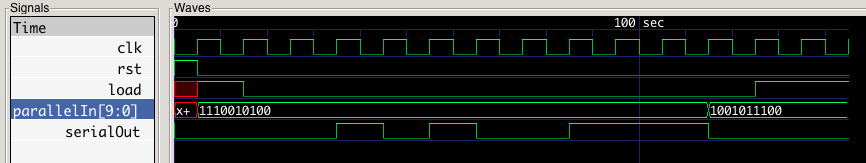
\includegraphics[width=0.75\linewidth]{figures/gtkwave/psShiftReg_gtkwave.png}
        \caption{psShiftReg module waveform}
        \label{fig:psShiftReg_gtkwave}
      \end{figure}

      % spShiftReg
      \begin{figure}[H]
        \centering
        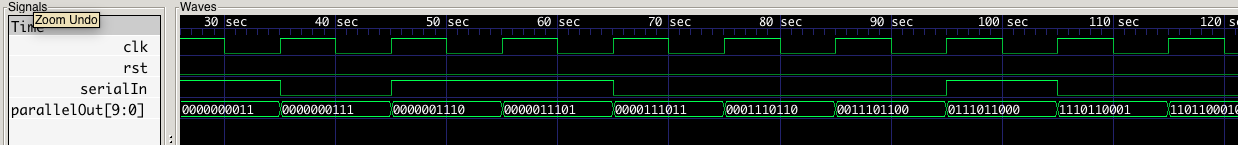
\includegraphics[width=0.75\linewidth]{figures/gtkwave/spShiftReg_gtkwave.png}
        \caption{spShiftReg module waveform}
        \label{fig:spShiftReg_gtkwave}
      \end{figure}

      % PISO
      \begin{figure}[H]
        \centering
        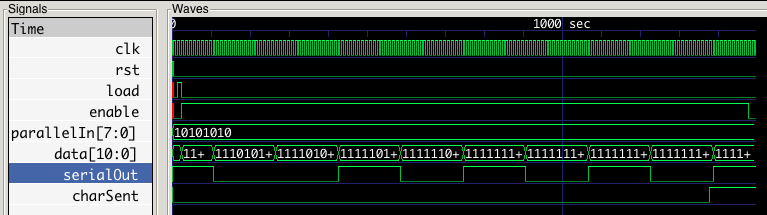
\includegraphics[width=0.75\linewidth]{figures/gtkwave/PISO_gtkwave.png}
        \caption{PISO module waveform}
        \label{fig:PISO_gtkwave}
      \end{figure}

      % SIPO
      \begin{figure}[H]
        \centering
        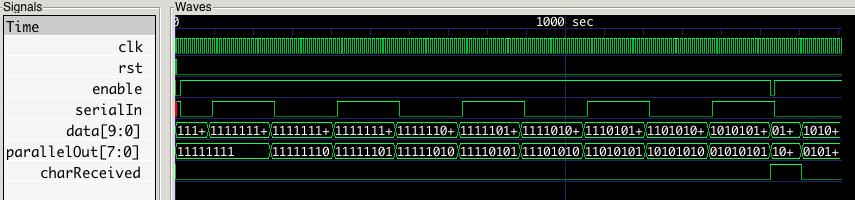
\includegraphics[width=0.75\linewidth]{figures/gtkwave/SIPO_gtkwave.png}
        \caption{SIPO module waveform}
        \label{fig:SIPO_gtkwave}
      \end{figure}

      % SPS_interface
      \begin{figure}[H]
        \centering
        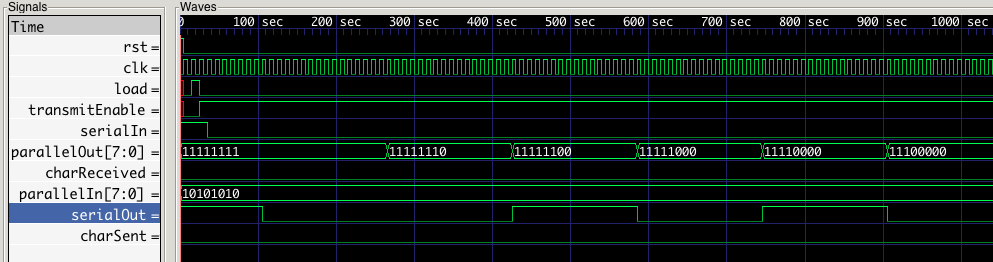
\includegraphics[width=0.75\linewidth]{figures/gtkwave/SPS_interface_gtkwave.png}
        \caption{SPS\_interface module waveform}
        \label{fig:SPS_interface_gtkwave}
      \end{figure}
\end{document}